\documentclass[11pt,a4paper]{article}  
\usepackage{graphicx}
\usepackage{polski}
\usepackage[utf8]{inputenc}
\usepackage{enumerate}
\usepackage{comment}
\usepackage[a4paper, left=2.5cm, right=2.5cm, top=2.5cm, bottom=2.5cm]{geometry}
\setlength{\headheight}{14pt}
\renewcommand{\baselinestretch}{1.18} 
\usepackage{fancyhdr}
\usepackage{hyperref}
\usepackage{indentfirst}
\usepackage{tabularx}
\usepackage{multirow}
\usepackage{float}
\usepackage{amsmath, amssymb, amsthm}
\usepackage{array}
\usepackage[export]{adjustbox}
\usepackage{icomma}
\usepackage{xcolor}
\usepackage{ tipa }
\usepackage{ gensymb }
\usepackage{ upgreek }
\usepackage{svg}
\usepackage{fancyvrb}
\usepackage{fvextra}

%Data w naglówku
\pagestyle{fancy}
\fancyhf{} 
\fancyhead[R]{\today} 

%Numer strony w stopce
\fancyhf{} 
\fancyfoot[C]{\thepage} 

\begin{document}
\noindent{\Huge\bfseries Podstawy Baz Danych }  \\\\
\noindent środa 16:45 \\
\noindent grupa nr. 1 \\\\
\textbf{Autorzy:}\\Maciej Kus - Widoki, Procedury, Funkcje, Dokumentacja\\Łukasz Krementowski - Procedury, Funkcje, Triggery, Uprawnienia, Dane\\Krzysztof Pieczka - Widoki, Procedury, Funkcje, Indeksy\\
\hrule

\section{Lista funkcji}

\subsection{Administrator bazy danych}
\begin{itemize}
    \item Modyfikowanie danych szkoleń
    \item Modyfikowanie danych użytkowników
\end{itemize}

\subsection{Gość}
\begin{itemize}
    \item Przeglądanie dostępnych szkoleń
    \item Możliwość założenia konta
\end{itemize}

\subsection{Student}
\begin{itemize}
    \item Przeglądanie dostępnych szkoleń
    \item Możliwość usunięcia konta
    \item Modyfikacja swoich danych osobowych
    \item Zapisanie się, zakup kursu
    \item Przeglądanie i dostęp do swoich szkoleń
    \item Zapisanie się na praktyki
    \item Zapisanie się na odrabianie nieobecności 
    \item Generowanie listy obecności
    \item Generowanie listy bilokacji
    \item Generowanie raportu o przebiegu studiów
    \item Generowanie harmonogramu
\end{itemize}

\subsection{Nauczyciel}
\begin{itemize}
    \item Przeglądanie własnych szkoleń
    \item Wyświetlanie listy studentów
    \item Wpisywanie obecności
    \item Generowanie list obecności
    \item Generowanie harmonogramu
\end{itemize}

\subsection{Dyrektor} 
\begin{itemize}
    \item Zmiana terminu płatności
    \item Generowanie raportów finansowych
    \item Generowanie raportów o wydarzeniach
    \item Generowanie raportów o frekwencji
    \item Generowanie list obecności       
    \item Generowanie list bilokacji
\end{itemize}

\subsection{Pracownik sekretariatu}
\begin{itemize}
    \item Dodawanie szkoleń
    \item Dodawanie pracowników
    \item Przypisywanie pracowników do szkoleń
    \item Modyfikacja szkoleń
    
\end{itemize}

\subsection{Tłumacz}
\begin{itemize}
    \item Dostęp do tłumaczonych kursów
    \item Generowanie harmonogramu
\end{itemize}

\section{Schemat i opis bazy danych}

\begin{figure}[H]
    \centering
    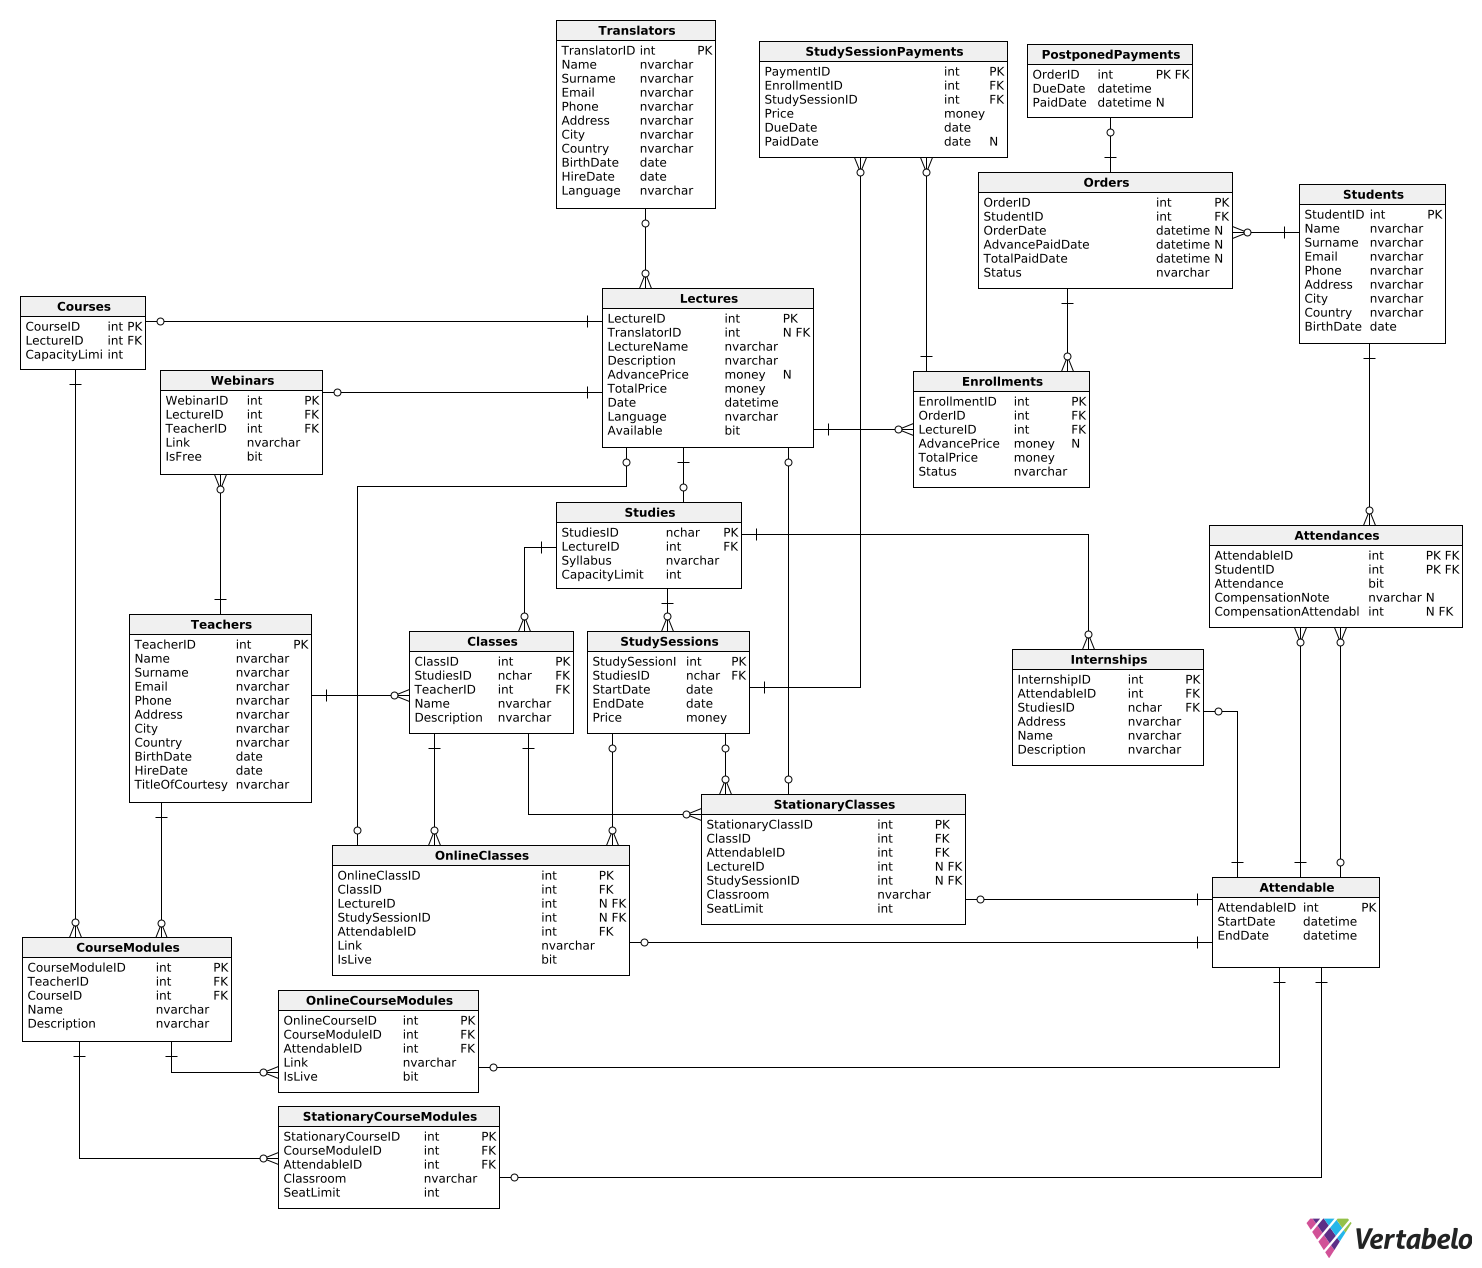
\includegraphics[scale=0.45, center]{scheme.png}
    \caption{Diagram schematu bazy danych}
    \label{fig:enter-label}
\end{figure}

\noindent W opisach tabel zostały użyte słowa kluczowe:
\begin{itemize}
    \item \textbf{szkolenie} (Lecture) - dowolna z oferowanych usług
    \item \textbf{zajęcia} (Attendable) - szkolenie, na którym prowadzona jest lista obecności
    \item \textbf{ćwiczenia} (Online/Stationary\ \ Classes/CourseModules) - zajęcia, które są częścią przedmiotu na studiach lub modułu kursu.
\end{itemize}

\newpage

\subsection{Students}
Zawiera informacje o studentach (posiadaczach konta).

\begin{itemize}
    \item[-] \textbf{StudentID int} - Identyfikator studenta
    \item[-] Name nvarchar - Imię studenta
    \item[-] Surname nvarchar - Nazwisko studenta
    \item[-] Emain nvarchar - Email studenta
    \item[-] Phone nvarchar - Numer telefonu studenta
    \item[-] Address nvarchar - Adres zamieszkania studenta
    \item[-] City nvarchar - Miasto zamieszkania studenta
    \item[-] Country nvarchar - Kraj zamieszkania studenta
    \item[-] Birthdate date - Data urodzenia studenta
\end{itemize}

\begin{Verbatim}[breaklines=true]
CREATE TABLE Students (
    StudentID int  NOT NULL IDENTITY(1,1),
    Name nvarchar(50)  NOT NULL,
    Surname nvarchar(50)  NOT NULL,
    Email nvarchar(100)  NOT NULL,
    Phone nvarchar(30)  NOT NULL,
    Address nvarchar(255)  NOT NULL,
    City nvarchar(50)  NOT NULL,
    Country nvarchar(69)  NOT NULL,
    BirthDate date  NOT NULL,

    CONSTRAINT Students_pk PRIMARY KEY (StudentID),

    CONSTRAINT UQ_Students_Email UNIQUE (Email),
    CONSTRAINT UQ_Students_Phone UNIQUE (Phone),
    CONSTRAINT CHK_Students_BirthDate CHECK (BirthDate < GETDATE() AND BirthDate > '1900-01-01')
);
\end{Verbatim}

Warunki integralnościowe:
\begin{itemize}
    \item Automatyczna inkrementacja StudentID.
    \item Email powinien być unikalny.
    \item Numer telefonu powinien być unikalny.
    \item Data urodzenia powinna być sensowna.
\end{itemize}

\subsection{Orders}
Zawiera informacje o zamówieniu. W zależności od statusu pełni rolę rozpoczętego zamówienia, zakończonego zamówienia, lub koszyka.

\begin{itemize}
    \item[-] \textbf{OrderID int} - Identyfikator zamówienia
    \item[-] \textit{StudentID int} - Identyfikator studenta
    \item[-] OrderDate date - Data rozpoczęcia zamówienia
    \item[-] AdvancePaidDate date - Data opłacenia zaliczki
    \item[-] TotalPaidDate date - Data opłacenia zamówienia w całości
    \item[-] Status nvarchar - Status płatności    
\end{itemize}

\begin{Verbatim}[breaklines=true]
CREATE TABLE Orders (
    OrderID int  NOT NULL IDENTITY(1,1),
    StudentID int  NOT NULL,
    OrderDate datetime  NULL DEFAULT NULL,
    AdvancePaidDate datetime  NULL DEFAULT NULL,
    TotalPaidDate datetime  NULL DEFAULT NULL,
    Status nvarchar(15)  NOT NULL,

    CONSTRAINT Orders_pk PRIMARY KEY (OrderID),
    CONSTRAINT Orders_Students FOREIGN KEY (StudentID) REFERENCES Students (StudentID),

    CONSTRAINT CHK_Orders_Status CHECK (Status IN ('Pending', 'Completed', 'Failed', 'Canceled', 'Cart'))
);
\end{Verbatim}

Warunki integralnościowe:
\begin{itemize}
    \item Automatyczna inkrementacja OrderID.
    \item Domyślnie daty nie są wpisywane (nie potrzebujemy daty koszyka).
    \item Sprawdzanie czy podany status jest dopuszczalny.
\end{itemize}

\subsection{PostponedPayments}
Zawiera informacje o opóźnieniach płatności udzielonych przez dyrektorów.

\begin{itemize}
    \item[-] \textbf{\textit{OrderID int}} - Identyfikator zamówienia
    \item[-] DueDate date - Wymagana data zapłaty należności
    \item[-] PaidDate date - Data opłacenia należności
\end{itemize}

\begin{Verbatim}[breaklines=true]
CREATE TABLE PostponedPayments (
    OrderID int  NOT NULL,
    DueDate datetime  NOT NULL,
    PaidDate datetime  NULL DEFAULT NULL,

    CONSTRAINT PostponedPayments_pk PRIMARY KEY (OrderID),
    CONSTRAINT PostponedPayments_Orders FOREIGN KEY (OrderID) REFERENCES Orders (OrderID),
    CONSTRAINT UQ_PostponedPayments_Orders UNIQUE (OrderID),

    CONSTRAINT CHK_PostponedPayments_DueDate CHECK (DueDate > GETDATE())
);
\end{Verbatim}

Warunki integralnościowe:
\begin{itemize}
    \item Wymagana data płatności powinna być w przyszłości.
\end{itemize}

\subsection{Enrollments}
Zawiera informacje o zapisie studenta na jeden z kursów.

\begin{itemize}
    \item[-] \textbf{EnrollmentID int} - Identyfikator zapisania
    \item[-] \textit{OrderID int} - Identyfikator zamówienia
    \item[-] \textit{LectureID int} - Identyfikator szkolenia
    \item[-] AdvancePrice money - Cena zapłacona za zaliczkę szkolenia
    \item[-] TotalPrice money - Całkowita cena zapłacona za szkolenie
    \item[-] Status nvarchar - Status studenta w szkoleniu    
\end{itemize}

\begin{Verbatim}[breaklines=true]
CREATE TABLE Enrollments (
    EnrollmentID int  NOT NULL IDENTITY(1,1),
    OrderID int  NOT NULL,
    LectureID int  NOT NULL,
    AdvancePrice money  NULL DEFAULT NULL,
    TotalPrice money  NOT NULL,
    Status nvarchar(20)  NOT NULL,

    CONSTRAINT Enrollments_pk PRIMARY KEY (EnrollmentID),
    CONSTRAINT Enrollments_Lectures FOREIGN KEY (LectureID) REFERENCES Lectures (LectureID),
    CONSTRAINT Enrollments_Orders FOREIGN KEY (OrderID) REFERENCES Orders (OrderID),

    CONSTRAINT CHK_Enrollments_Status CHECK (Status IN ('Completed', 'Failed', 'InProgress', 'Resigned', 'AwaitingPayment', 'NotPaidOnTime'))
);
\end{Verbatim}

Warunki integralnościowe:
\begin{itemize}
    \item Automatyczna inkrementacja EnrollmentID.
    \item Domyślnie szkolenie nie ma zaliczki.
    \item Sprawdzenie czy podany status jest dopuszczalny.
\end{itemize}

\subsection{StudySessionPayments}
Zawiera informacje o płatnościach za zjazdy.

\begin{itemize}
    \item[-] \textbf{PaymentID int} - Identyfikator płatności
    \item[-] \textit{EnrollmentID int} - Identyfikator zapisania
    \item[-] \textit{StudySessionID int} - Identyfikator zjazdu
    \item[-] Price money - Cena za zjazd
    \item[-] DueDate date - Wymagana data opłacenia należności    
    \item[-] PaidDate date - Data opłacenia należności    
\end{itemize}

\begin{Verbatim}[breaklines=true]
CREATE TABLE StudySessionPayments (
    PaymentID int  NOT NULL IDENTITY(1,1),
    EnrollmentID int  NOT NULL,
    StudySessionID int  NOT NULL,  
    Price money  NOT NULL,
    DueDate date  NOT NULL,
    PaidDate date  NULL DEFAULT NULL,

    CONSTRAINT StudySessionPayments_pk PRIMARY KEY (PaymentID),
    CONSTRAINT StudySessionPayments_Enrollments FOREIGN KEY (EnrollmentID) REFERENCES Enrollments (EnrollmentID),
    CONSTRAINT StudySessionPayments_StudySession FOREIGN KEY (StudySessionID) REFERENCES StudySessions (StudySessionID),

    CONSTRAINT CHK_StudySessionPayments_DueDate CHECK (DueDate > GETDATE())
);
\end{Verbatim}

Warunki integralnościowe:
\begin{itemize}
    \item Automatyczna inkrementacja PaymentID.
    \item Wymagana data płatności powinna być w przyszłości.
\end{itemize}

\subsection{Attendances}
Zawiera informacje o obecnościach studentów.

\begin{itemize}
    \item[-] \textbf{\textit{AttendableID int}} - Identyfikator zajęć
    \item[-] \textbf{\textit{StudentID int}} - Identyfikator studenta 
    \item[-] Attendance bit - Obecność na zajęciach
    \item[-] CompensationNote nvarchar - Notatka wyjaśniająca odrobienie zajęć
    \item[-] \textit{ CompensationAttendableID int} - Identyfikator zajęć odrabiających nieobecność 
\end{itemize}

\begin{Verbatim}[breaklines=true]
CREATE TABLE Attendances (
    AttendableID int  NOT NULL,
    StudentID int  NOT NULL,
    Attendance bit  NOT NULL DEFAULT 1,
    CompensationNote nvarchar(MAX)  NULL DEFAULT NULL,
    CompensationAttendableID int  NULL DEFAULT NULL,

    CONSTRAINT Attendances_pk PRIMARY KEY (AttendableID,StudentID),
    CONSTRAINT Attendances_Attendable FOREIGN KEY (AttendableID) REFERENCES Attendable (AttendableID),
    CONSTRAINT Attendances_Students FOREIGN KEY (StudentID) REFERENCES Students (StudentID),
    CONSTRAINT Attendances_AttendableCompensation FOREIGN KEY (CompensationAttendableID) REFERENCES Attendable (AttendableID)
);
\end{Verbatim}

Warunki integralnościowe:
\begin{itemize}
    \item Domyślnie wpisywana jest obecność.
    \item Odrobienie zajęć domyślnie nie występuje.
\end{itemize}

\subsection{Attendable}
Zawiera informacje o szkoleniach wymagających obecności.

\begin{itemize}
    \item[-] \textbf{AttendableID int} - Identyfikator zajęć 
    \item[-] StartDate datetime - Data rozpoczęcia zajęć
    \item[-] EndDate datetime - Data zakończenia zajęć
\end{itemize}

\begin{Verbatim}[breaklines=true]
CREATE TABLE Attendable (
    AttendableID int  NOT NULL IDENTITY(1,1),
    StartDate date  NOT NULL,
    EndDate date  NOT NULL,

    CONSTRAINT Attendable_pk PRIMARY KEY (AttendableID),

    CONSTRAINT CHK_Attendable_Date CHECK (StartDate < EndDate)
);
\end{Verbatim}

Warunki integralnościowe:
\begin{itemize}
    \item Automatyczna inkrementacja AttendableID.
    \item Zajęcia rozpoczynają się wcześniej niż się kończą.
\end{itemize}

\subsection{Lectures}
Zawiera informacje o szkoleniach każdego rodzaju.

\begin{itemize}
    \item[-] \textbf{LectureID int} - Identyfikator szkolenia
    \item[-] \textit{TranslatorID int} - Tłumacz szkolenia
    \item[-] LectureName nvarchar - Nazwa szkolenia
    \item[-] Description nvarchar - Opis szkolenia
    \item[-] AdvancePrice money - Aktualna cena zaliczki szkolenia
    \item[-] TotalPrice money - Aktualna całkowita cena szkolenia
    \item[-] Date datetime - Data rozpoczęcia szkolenia
    \item[-] Language nvarchar - Język w którym jest prowadzone szkolenie
    \item[-] Available bit - Dostępność kursu do zakupu
\end{itemize}

\begin{Verbatim}[breaklines=true]
CREATE TABLE Lectures (
    LectureID int  NOT NULL IDENTITY(1,1),
    TranslatorID int  NULL DEFAULT NULL,
    LectureName nvarchar(100)  NOT NULL,
    Description nvarchar(MAX)  NOT NULL,
    AdvancePrice money NULL DEFAULT NULL,
    TotalPrice money  NOT NULL,
    Date datetime  NOT NULL,
    Language nvarchar(10)  NOT NULL DEFAULT 'pl',
    Available bit NOT NULL DEFAULT 0,

    CONSTRAINT LectureID PRIMARY KEY (LectureID),
    CONSTRAINT Lectures_Translators FOREIGN KEY (TranslatorID) REFERENCES Translators (TranslatorID),

    CONSTRAINT CHK_Lectures_TotalPrice CHECK (TotalPrice >= 0),
    CONSTRAINT CHK_Lectures_AdvancePrice CHECK (AdvancePrice is NULL OR AdvancePrice >= 0),
    CONSTRAINT CHK_Lectures_Date CHECK (Date >= GETDATE())
);
\end{Verbatim}

Warunki integralnościowe:
\begin{itemize}
    \item Automatyczna inkrementacja LectureID.
    \item Domyślnie tłumacz nie jest przypisywany.
    \item Domyślnie szkolenie nie ma zaliczki.
    \item Domyślnie szkolenie jest prowadzone po polsku.
    \item Domyślnie szkolenie nie jest dostępne do zakupu (przed    wprowadzeniem go w całości do bazy danych).
    \item Ceny powinny być dodatnie.
    \item Data rozpoczęcia powinna być w przyszłości.
\end{itemize}

\subsection{Teachers}
Zawiera informacje o prowadzących zajęcia.

\begin{itemize}
    \item[-] \textbf{TeacherID int} - Identyfikator prowadzącego
    \item[-] Name nvarchar - Imię prowadzącego
    \item[-] Surname nvarchar - Nazwisko prowadzącego
    \item[-] Emain nvarchar - Email prowadzącego
    \item[-] Phone nvarchar - Numer telefonu prowadzącego
    \item[-] Address nvarchar - Adres zamieszkania prowadzącego
    \item[-] City nvarchar - Miasto zamieszkania prowadzącego
    \item[-] Country nvarchar - Kraj zamieszkania prowadzącego
    \item[-] Birthdate date - Data urodzenia prowadzącego
    \item[-] HireDate date - Data zatrudnienia prowadzącego
    \item[-] TitleOfCourtesy nvarchar - Tytuł naukowy prowadzącego
\end{itemize}

\begin{Verbatim}[breaklines=true]
CREATE TABLE Teachers (
    TeacherID int  NOT NULL IDENTITY(1,1),
    Name nvarchar(50)  NOT NULL,
    Surname nvarchar(50)  NOT NULL,
    Email nvarchar(100)  NOT NULL,
    Phone nvarchar(30)  NOT NULL,
    Address nvarchar(255)  NOT NULL,
    City nvarchar(50)  NOT NULL,
    Country nvarchar(69)  NOT NULL,
    BirthDate date  NOT NULL,
    HireDate date  NOT NULL,
    TitleOfCourtesy nvarchar(20)  NOT NULL,

    CONSTRAINT Teachers_pk PRIMARY KEY (TeacherID),

    CONSTRAINT UQ_Teachers_Email UNIQUE (Email),
    CONSTRAINT UQ_Teachers_Phone UNIQUE (Phone),
    CONSTRAINT CHK_Teachers_BirthDate CHECK (BirthDate < GETDATE() AND BirthDate > '1900-01-01'),
    CONSTRAINT CHK_Teachers_HireDate CHECK (HireDate < GETDATE() AND HireDate > BirthDate)
);
\end{Verbatim}

Warunki integralnościowe:
\begin{itemize}
    \item Automatyczna inkrementacja TeacherID.
    \item Email powinien być unikalny.
    \item Numer telefonu powinien być unikalny.
    \item Data urodzenia powinna być sensowna.
    \item Data zatrudnienia powinna być sensowna.
\end{itemize}

\subsection{Translators}
Zawiera informacje o tłumaczach.

\begin{itemize}
    \item[-] \textbf{TranslatorID int} - Identyfikator tłumacza
    \item[-] Name nvarchar - Imię tłumacza
    \item[-] Surname nvarchar - Nazwisko tłumacza
    \item[-] Emain nvarchar - Email tłumacza
    \item[-] Phone nvarchar - Numer telefonu tłumacza
    \item[-] Address nvarchar - Adres zamieszkania tłumacza
    \item[-] City nvarchar - Miasto zamieszkania tłumacza
    \item[-] Country nvarchar - Kraj zamieszkania tłumacza
    \item[-] Birthdate date - Data urodzenia tłumacza
    \item[-] HireDate date - Data zatrudnienia tłumacza
    \item[-] Language nvarchar - Język którym operuje tłumacz
\end{itemize}

\begin{Verbatim}[breaklines=true]
CREATE TABLE Translators (
    TranslatorID int  NOT NULL IDENTITY(1,1),
    Name nvarchar(50)  NOT NULL,
    Surname nvarchar(50)  NOT NULL,
    Email nvarchar(100)  NOT NULL,
    Phone nvarchar(30)  NOT NULL,
    Address nvarchar(255)  NOT NULL,
    City nvarchar(50)  NOT NULL,
    Country nvarchar(69)  NOT NULL,
    BirthDate date  NOT NULL,
    HireDate date  NOT NULL,
    Language nvarchar(10)  NOT NULL,

    CONSTRAINT Translators_pk PRIMARY KEY (TranslatorID),

    CONSTRAINT UQ_Translators_Email UNIQUE (Email),
    CONSTRAINT UQ_Translators_Phone UNIQUE (Phone),
    CONSTRAINT CHK_Translators_BirthDate CHECK (BirthDate < GETDATE() AND BirthDate > '1900-01-01'),
    CONSTRAINT CHK_Translators_HireDate CHECK (HireDate < GETDATE())
);
\end{Verbatim}

Warunki integralnościowe:
\begin{itemize}
    \item Automatyczna inkrementacja TranslatorID.
    \item Email powinien być unikalny.
    \item Numer telefonu powinien być unikalny.
    \item Data urodzenia powinna być sensowna.
    \item Data zatrudnienia powinna być sensowna.
\end{itemize}

\subsection{Webinars}
Zawiera informacje o webinarach.

\begin{itemize}
    \item[-] \textbf{WebinarID int} - Identyfikator webinaru
    \item[-] \textit{LectureID int} - Identyfikator szkolenia
    \item[-] \textit{TeacherID int} - Identyfikator prowadzącego
    \item[-] Link nvarchar - Link do webinaru
    \item[-] IsFree bit - Informacja czy webinar jest darmowy (ogólnodostępny)
\end{itemize}

\begin{Verbatim}[breaklines=true]
CREATE TABLE Webinars (
    WebinarID int  NOT NULL IDENTITY(1,1),
    LectureID int  NOT NULL,
    TeacherID int  NOT NULL,
    Link nvarchar(MAX)  NOT NULL,
    IsFree bit  NOT NULL,

    CONSTRAINT Webinars_pk PRIMARY KEY  (WebinarID),
    CONSTRAINT Webinars_Teachers FOREIGN KEY (TeacherID) REFERENCES Teachers (TeacherID),
    CONSTRAINT Webinars_Lectures FOREIGN KEY (LectureID) REFERENCES Lectures (LectureID),
    CONSTRAINT UQ_Webinars_Lectures UNIQUE (LectureID)
);
\end{Verbatim}

Warunki integralnościowe:
\begin{itemize}
    \item Automatyczna inkrementacja WebinarID.
\end{itemize}

\subsection{Courses}
Zawiera informacje o kursach.

\begin{itemize}
    \item[-] \textbf{CourseID int} - Identyfikator kursu
    \item[-] \textit{LectureID int} - Identyfikator szkolenia
    \item[-] CapacityLimit int - Limit miejsc na kursie
\end{itemize}

\begin{Verbatim}[breaklines=true]
CREATE TABLE Courses (
    CourseID int  NOT NULL IDENTITY(1,1),
    LectureID int  NOT NULL,
    CapacityLimit int NOT NULL,

    CONSTRAINT Courses_pk PRIMARY KEY (CourseID),
    CONSTRAINT Courses_Lectures FOREIGN KEY (LectureID) REFERENCES Lectures (LectureID),
    CONSTRAINT UQ_Courses_Lectures UNIQUE (LectureID),

    CONSTRAINT CHK_Courses_CapacityLimit CHECK (CapacityLimit > 0)
);
\end{Verbatim}

Warunki integralnościowe:
\begin{itemize}
    \item Automatyczna inkrementacja CourseID.
    \item Limit miejsc powinien być dodatni.
\end{itemize}

\subsection{CourseModules}
Zawiera informacje o modułach kursów.

\begin{itemize}
    \item[-] \textbf{CourseModuleID int} - Identyfikator modułu
    \item[-] \textit{TeacherID int} - Identyfikator prowadzącego
    \item[-] \textit{CourseID int} - Identyfikator kursu
    \item[-] Name nvarchar - Nazwa modułu 
    \item[-] Description nvarchar - Opis modułu 
\end{itemize}

\begin{Verbatim}[breaklines=true]
CREATE TABLE CourseModules (
    CourseModuleID int  NOT NULL IDENTITY(1,1),
    TeacherID int  NOT NULL,
    CourseID int  NOT NULL,
    Name nvarchar(100)  NOT NULL,
    Description nvarchar(MAX)  NOT NULL,

    CONSTRAINT CourseModules_pk PRIMARY KEY (CourseModuleID),
    CONSTRAINT CourseModules_Courses FOREIGN KEY (CourseID) REFERENCES Courses (CourseID),
    CONSTRAINT CourseModules_Teachers FOREIGN KEY (TeacherID) REFERENCES Teachers (TeacherID)
);
\end{Verbatim}

Warunki integralnościowe:
\begin{itemize}
    \item Automatyczna inkrementacja CourseModuleID.
\end{itemize}

\subsection{StationaryCourseModules}
Zawiera informacje o stacjonarnych ćwiczeniach dla modułu kursu.

\begin{itemize}
    \item[-] \textbf{StationaryCourseID int} - Identyfikator ćwiczeń stacjonarnych
    \item[-] \textit{CourseModuleID int} - Identyfikator modułu
    \item[-] \textit{AttendableID int} - Identyfikator zajęć
    \item[-] Classroom nvarchar - Numer sali
    \item[-] SeatLimit int - Limit miejsc w module
\end{itemize}

\begin{Verbatim}[breaklines=true]
CREATE TABLE StationaryCourseModules (
    StationaryCourseID int  NOT NULL IDENTITY(1,1),
    CourseModuleID int  NOT NULL,
    AttendableID int  NOT NULL,
    Classroom nvarchar(10)  NOT NULL,
    SeatLimit int  NOT NULL,

    CONSTRAINT StationaryCourseModules_pk PRIMARY KEY (StationaryCourseID),
    CONSTRAINT StationaryCourseModules_CourseModules FOREIGN KEY (CourseModuleID) REFERENCES CourseModules (CourseModuleID),
    CONSTRAINT StationaryCourseModules_Attendable FOREIGN KEY (AttendableID) REFERENCES Attendable (AttendableID),
    CONSTRAINT UQ_StationaryCourseModules_AttendableID UNIQUE (AttendableID),
    CONSTRAINT CHK_StationaryCourseModules_SeatLimit CHECK (SeatLimit > 0)
);
\end{Verbatim}

Warunki integralnościowe:
\begin{itemize}
    \item Automatyczna inkrementacja StationaryCourseID.
    \item Liczba miejsc powinna być dodatnia.
    \item Klucz obcy AttendableID jest unikalny w tabeli.
\end{itemize}

\subsection{OnlineCourseModules}
Zawiera informacje o ćwiczeniach online dla modułu kursu.

\begin{itemize}
    \item[-] \textbf{OnlineCourseID int} - Identyfikator ćwiczeń online
    \item[-] \textit{CourseModuleID int} - Identyfikator modułu
    \item[-] \textit{AttendableID int} - Identyfikator zajęć
    \item[-] Link nvarchar - Link do spotkania
    \item[-] IsLive bit - Czy spotkanie jest na żywo
\end{itemize}

\begin{Verbatim}[breaklines=true]
CREATE TABLE OnlineCourseModules (
    OnlineCourseID int  NOT NULL IDENTITY(1,1),
    CourseModuleID int  NOT NULL,
    AttendableID int  NOT NULL,
    Link nvarchar(MAX)  NOT NULL,
    IsLive bit  NOT NULL,

    CONSTRAINT OnlineCourseModules_pk PRIMARY KEY  (OnlineCourseID),
    CONSTRAINT OnlineCourseModules_CourseModules FOREIGN KEY (CourseModuleID) REFERENCES CourseModules (CourseModuleID),
    CONSTRAINT OnlineCourseModules_Attendable FOREIGN KEY (AttendableID) REFERENCES Attendable (AttendableID),
    CONSTRAINT UQ_OnlineCourseModules_AttendableID UNIQUE (AttendableID)
);
\end{Verbatim}

Warunki integralnościowe:
\begin{itemize}
    \item Automatyczna inkrementacja OnlineCourseID.
    \item Klucz obcy AttendableID jest unikalny w tabeli.
\end{itemize}

\subsection{Studies}
Zawiera informacje o studiach.

\begin{itemize}
    \item[-] \textbf{StudiesID nchar} - Identyfikator studiów
    \item[-] \textit{LectureID int} - Identyfikator szkolenia
    \item[-] Syllabus nvarchar - Sylabus studiów
    \item[-] CapacityLimit int - Limit miejsc na studiach
\end{itemize}

\begin{Verbatim}[breaklines=true]
CREATE TABLE Studies (
    StudiesID nchar(5)  NOT NULL,
    LectureID int  NOT NULL,
    Syllabus nvarchar(MAX)  NOT NULL,
    CapacityLimit int  NOT NULL,

    CONSTRAINT Studies_pk PRIMARY KEY (StudiesID),
    CONSTRAINT Studies_Lectures FOREIGN KEY (LectureID) REFERENCES Lectures (LectureID),
    CONSTRAINT UQ_Studies_Lectures UNIQUE (LectureID),
    
    CONSTRAINT CHK_Studies_CapacityLimit CHECK (CapacityLimit > 0)
);
\end{Verbatim}

Warunki integralnościowe:
\begin{itemize}
    \item Limit miejsc powinien być dodatni.
\end{itemize}

\subsection{StudySessions}
Zawiera informacje o zjazdach na studiach.

\begin{itemize}
    \item[-] \textbf{StudySessionID int} - Identyfikator zjazdy
    \item[-] \textit{StudiesID nchar} - Identyfikator studiów
    \item[-] StartDate date - Data rozpoczęcia zjazdu
    \item[-] EndDate date - Data zakończenia zjazdu
    \item[-] Price money - Koszt zjazdu
\end{itemize}

\begin{Verbatim}[breaklines=true]
CREATE TABLE StudySessions (
    StudySessionID int  NOT NULL IDENTITY(1,1),
    StudiesID nchar(5)  NOT NULL,
    StartDate date  NOT NULL,
    EndDate date  NOT NULL,
    Price money  NOT NULL,

    CONSTRAINT StudySessions_pk PRIMARY KEY (StudySessionID),
    CONSTRAINT StudySessions_Studies FOREIGN KEY (StudiesID) REFERENCES Studies (StudiesID),

    CONSTRAINT CHK_StudySessions_Date CHECK (StartDate < EndDate),
    CONSTRAINT CHK_StudySessions_Price CHECK (Price >= 0),
);
\end{Verbatim}

Warunki integralnościowe:
\begin{itemize}
    \item Cena powinna być dodatnia.
    \item Zjazd rozpoczyna się wcześniej niż się kończy.
\end{itemize}

\subsection{Classes}
Zawiera informacje o przedmiotach.

\begin{itemize}
    \item[-] \textbf{ClassID int} - Identyfikator przedmiotu
    \item[-] \textit{StudiesID nchar} - Identyfikator studiów
    \item[-] \textit{TeacherID int} - Identyfikator prowadzącego
    \item[-] Name nvarchar - Nazwa przedmiotu
    \item[-] Description nvarchar - Opis przedmiotu
\end{itemize}

\begin{Verbatim}[breaklines=true]
CREATE TABLE Classes (
    ClassID int  NOT NULL IDENTITY(1,1),
    StudiesID nchar(5)  NOT NULL,
    TeacherID int  NOT NULL,
    Name nvarchar(100)  NOT NULL,
    Description nvarchar(MAX)  NOT NULL,

    CONSTRAINT Classes_pk PRIMARY KEY (ClassID),
    CONSTRAINT Classes_Teachers FOREIGN KEY (TeacherID) REFERENCES Teachers (TeacherID),
    CONSTRAINT Classes_Studies FOREIGN KEY (StudiesID) REFERENCES Studies (StudiesID)
);
\end{Verbatim}

Warunki integralnościowe:
\begin{itemize}
    \item Automatyczna inkrementacja ClassID.
\end{itemize}

\subsection{OnlineClasses}
Zawiera informacje o ćwiczeniach online z przedmiotu.

\begin{itemize}
    \item[-] \textbf{OnlineClassID int} - Identyfikator ćwiczeń online
    \item[-] \textit{ClassID int} - Identyfikator ćwiczeń
    \item[-] \textit{AttendableID int} - Identyfikator zajęć
    \item[-] \textit{LectureID int} - Identyfikator szkolenia - jeśli ćwiczenia są dostępne do osobnego zakupu
    \item[-] \textit{StudySessionID int} - Identyfikator zjazdu - jeśli ćwiczenia należą do zjazdu
    \item[-] Link nvarchar - Link do ćwiczeń
    \item[-] isLive bit - Czy ćwiczenia są na żywo
\end{itemize}

\begin{Verbatim}[breaklines=true]
CREATE TABLE OnlineClasses (
    OnlineClassID int  NOT NULL IDENTITY(1,1),
    ClassID int  NOT NULL,
    AttendableID int  NOT NULL,
    LectureID int NULL DEFAULT NULL,
    StudySessionID int NULL DEFAULT NULL,
    Link nvarchar(MAX)  NOT NULL,
    IsLive bit  NOT NULL,

    CONSTRAINT OnlineClasses_pk PRIMARY KEY (OnlineClassID),
    CONSTRAINT OnlineClasses_Classes FOREIGN KEY (ClassID) REFERENCES Classes (ClassID),
    CONSTRAINT OnlineClasses_Attendable FOREIGN KEY (AttendableID) REFERENCES Attendable (AttendableID),
    CONSTRAINT OnlineClasses_Lectures FOREIGN KEY (LectureID) REFERENCES Lectures (LectureID),
    CONSTRAINT OnlineClasses_StudySessions FOREIGN KEY (StudySessionID) REFERENCES StudySessions (StudySessionID),
    CONSTRAINT UQ_OnlineClasses_AttendableID UNIQUE (AttendableID)
);
\end{Verbatim}

Warunki integralnościowe:
\begin{itemize}
    \item Automatyczna inkrementacja OnlineClassID.
    \item Domyślnie ćwiczenia nie są dostępne do osobnego zakupu.
    \item Klucz obcy AttendableID jest unikalny w tabeli.
\end{itemize}

\subsection{StationaryClasses}
Zawiera informacje o ćwiczeniach stacjonarnych z przedmiotu.

\begin{itemize}
    \item[-] \textbf{StationaryClassID int} - Identyfikator ćwiczeń stacjonarnych
    \item[-] \textit{ClassID int} - Identyfikator ćwiczeń
    \item[-] \textit{AttendableID int} - Identyfikator zajęć
    \item[-] \textit{LectureID int} - Identyfikator szkolenia - jeśli ćwiczenia są dostępne do osobnego zakupu
    \item[-] \textit{StudySessionID int} - Identyfikator zjazdu - jeśli ćwiczenia należą do zjazdu
    \item[-] Classroom nvarchar - Numer sali
    \item[-] SeatLimit int - Limit miejsc na ćwiczeniach
\end{itemize}

\begin{Verbatim}[breaklines=true]
CREATE TABLE StationaryClasses (
    StationaryClassID int  NOT NULL IDENTITY(1,1),
    ClassID int  NOT NULL,
    AttendableID int  NOT NULL,
    LectureID int NULL DEFAULT NULL,
    StudySessionID int NULL DEFAULT NULL,
    Classroom nvarchar(10)  NOT NULL,
    SeatLimit int  NOT NULL,

    CONSTRAINT StationaryClasses_pk PRIMARY KEY (StationaryClassID),
    CONSTRAINT StationaryClasses_Classes FOREIGN KEY (ClassID) REFERENCES Classes (ClassID),
    CONSTRAINT StationaryClasses_Attendable FOREIGN KEY (AttendableID) REFERENCES Attendable (AttendableID),
    CONSTRAINT StationaryClasses_Lectures FOREIGN KEY (LectureID) REFERENCES Lectures (LectureID),
    CONSTRAINT StationaryClasses_StudySessions FOREIGN KEY (StudySessionID) REFERENCES StudySessions (StudySessionID),
    CONSTRAINT UQ_StationaryClasses_AttendableID UNIQUE (AttendableID),
    CONSTRAINT CHK_StationaryClasses_SeatLimit CHECK (SeatLimit > 0)
);
\end{Verbatim}

Warunki integralnościowe:
\begin{itemize}
    \item Automatyczna inkrementacja StationaryClassID.
    \item Domyślnie ćwiczenia nie są dostępne do osobnego zakupu.
    \item Liczba miejsc powinna być dodatnia.
    \item Klucz obcy AttendableID jest unikalny w tabeli.
\end{itemize}

\subsection{Internships}
Zawiera informacje o praktykach.

\begin{itemize}
    \item[-] \textbf{InternshipID int} - Identyfikator praktyk
    \item[-] \textit{AttendableID int} - Identyfikator zajęć
    \item[-] \textit{StudiesID nchar} - Identyfikator studiów
    \item[-] Address nvarchar - Adres praktyki
    \item[-] Name nvarchar - Nazwa praktyki
    \item[-] Description nvarchar - Opis praktyki
\end{itemize}

\begin{Verbatim}[breaklines=true]
CREATE TABLE Internships (
    InternshipID int  NOT NULL IDENTITY(1,1),
    AttendableID int  NOT NULL,
    StudiesID nchar(5)  NOT NULL,
    Address nvarchar(255)  NOT NULL,
    Name nvarchar(100)  NOT NULL,
    Description nvarchar(MAX)  NOT NULL,

    CONSTRAINT Internships_pk PRIMARY KEY (InternshipID),
    CONSTRAINT Internships_Attendable FOREIGN KEY (AttendableID) REFERENCES Attendable (AttendableID),
    CONSTRAINT Internships_Studies FOREIGN KEY (StudiesID) REFERENCES Studies (StudiesID),
    CONSTRAINT UQ_Internships_AttendableID UNIQUE (AttendableID)
);
\end{Verbatim}

Warunki integralnościowe:
\begin{itemize}
    \item Automatyczna inkrementacja InternshipID.
    \item Klucz obcy AttendableID jest unikalny w tabeli.
\end{itemize}

\section{Widoki}
\subsection{Listy obecności na szkoleniach}

\subsubsection{Widok pomocniczy}
Zbiera razem obecności każdego studenta.
\begin{Verbatim}[breaklines=true]
create view VW_All_Attendance as
select D.AttendableID, D.StartDate, D.EndDate, S.StudentID, S.Name, S.Surname, A.Attendance, A.CompensationAttendableID
from Attendances A inner join Students S on S.StudentID = A.StudentID
    inner join Attendable D on D.AttendableID = A.AttendableID;
go
\end{Verbatim}

\subsubsection{Lista obecności na praktykach}
Przedstawia dla każdej praktyki i każdego zapisanego na nią studenta, informację czy był on na niej obecny.
\begin{Verbatim}[breaklines=true]
create view VW_Internships_Attendance as
select I.InternshipID, I.StudiesID, I.Address, I.Name InternshipName, I.Description, A.*
from VW_All_Attendance A inner join Internships I on I.AttendableID = A.AttendableID;
go
\end{Verbatim}

\subsubsection{Lista obecności na ćwiczeniach stacjonarnych z przedmiotów}
Przedstawia dla każdego ćwiczenia i każdego zapisanego na nie studenta, informację czy był on na nich obecny.
\begin{Verbatim}[breaklines=true]
create view VW_StationaryClasses_Attendance as
select C.StationaryClassID, C.ClassID, C.StudySessionID, C.Classroom, S.TeacherID, S.Name ClassName, S.Description, A.*
from VW_All_Attendance A inner join StationaryClasses C on C.AttendableID = A.AttendableID
    inner join Classes S on S.ClassID = C.ClassID;
go
\end{Verbatim}

\subsubsection{Lista obecności na ćwiczeniach online z przedmiotów}
Przedstawia dla każdego ćwiczenia i każdego zapisanego na nie studenta, informację czy był on na nich obecny.
\begin{Verbatim}[breaklines=true]
create view VW_OnlineClasses_Attendance as
select C.OnlineClassID, C.ClassID, C.StudySessionID, C.IsLive, S.TeacherID, S.Name ClassName, S.Description, A.*
from VW_All_Attendance A inner join OnlineClasses C on C.AttendableID = A.AttendableID
    inner join Classes S on S.ClassID = C.ClassID;
go
\end{Verbatim}

\subsubsection{Lista obecności na ćwiczeniach stacjonarnych modułów}
Przedstawia dla każdego ćwiczenia i każdego zapisanego na nie studenta, informację czy był on na nich obecny.
\begin{Verbatim}[breaklines=true]
create view VW_StationaryCourseModules_Attendance as
select M.StationaryCourseID, M.Classroom, C.CourseModuleID, C.CourseID, C.TeacherID, C.Name CourseName, C.Description, A.*
from VW_All_Attendance A inner join StationaryCourseModules M on M.AttendableID = A.AttendableID
    inner join CourseModules C on C.CourseModuleID = M.CourseModuleID;
go
\end{Verbatim}

\subsubsection{Lista obecności na ćwiczeniach online modułów}
Przedstawia dla każdego ćwiczenia i każdego zapisanego na nie studenta, informację czy był on na nich obecny.
\begin{Verbatim}[breaklines=true]
create view VW_OnlineCourseModules_Attendance as
select M.OnlineCourseID, M.IsLive, C.CourseModuleID, C.CourseID, C.TeacherID, C.Name CourseName, C.Description, A.*
from VW_All_Attendance A inner join OnlineCourseModules M on M.AttendableID = A.AttendableID
    inner join CourseModules C on C.CourseModuleID = M.CourseModuleID;
go
\end{Verbatim}

\subsection{Raport frekwencji na zakończonych wydarzeniach}
Poniższe widoki przedstawiają informacje o frekwencji na zakończonych wydarzeniach. \\ Zawiera się w tym ID spotkania, czas początku i końca, liczbę wszystkich zapisanych na niego studentów, liczbę obecnych studentów, procentową frekwencję (Obecni/Zapisani $\cdot 100\%$), oraz wszystkie informacje związane z tym wydarzeniem.
\subsubsection{Widok pomocniczy}
Przedstawia raport frekwencji dla każdego typu wydarzenia.
\begin{Verbatim}[breaklines=true]
create view VW_All_Attendance_Summary as
select A.AttendableID, A.StartDate, A.EndDate, count(A.StudentID) TotalStudents, sum(case when A.Attendance = 1 then 1 else 0 end) as PresentStudents,
    round( cast(sum(case when A.Attendance = 1 then 1 else 0 end) as float) / count(A.StudentID) * 100, 2 ) as AttendanceRate
from VW_All_Attendance A 
where A.EndDate < getdate()
group by A.AttendableID, A.StartDate, A.EndDate
go    
\end{Verbatim}

\subsubsection{Frekwencja na ćwiczeniach online z modułów kursów}
\begin{Verbatim}[breaklines=true]
create view VW_OnlineCourseModules_Attendance_Summary as
select A.attendableid, totalstudents, presentstudents, attendancerate, OCM.OnlineCourseID, CM.CourseModuleID, CourseID, Link, IsLive, TeacherID, Name, Description
    from VW_All_Attendance_Summary A
             inner join OnlineCourseModules OCM on A.attendableid = OCM.AttendableID
             inner join dbo.CourseModules CM on OCM.CourseModuleID = CM.CourseModuleID;
go  
\end{Verbatim}

\subsubsection{Frekwencja na ćwiczeniach stacjonarnych z modułów kursów}
\begin{Verbatim}[breaklines=true]
create view VW_StationaryCourseModules_Attendance_Summary as
select A.attendableid, totalstudents, presentstudents, attendancerate, SCM.StationaryCourseID, CourseID, CM.CourseModuleID, Classroom, SeatLimit,  TeacherID, CourseID, Name, Description
from VW_All_Attendance_Summary A
             inner join StationaryCourseModules SCM on A.attendableid = SCM.AttendableID
inner join dbo.CourseModules CM on SCM.CourseModuleID = CM.CourseModuleID
go
\end{Verbatim}

\subsubsection{Frekwencja na ćwiczeniach online z przedmiotów}
\begin{Verbatim}[breaklines=true]
create view VW_OnlineClasses_Attendance_Summary as
select A.attendableid, totalstudents, presentstudents, attendancerate, OC.OnlineClassID, OC.ClassID, StudySessionID, Link, IsLive, StudiesID, TeacherID, Name, Description
    from VW_All_Attendance_Summary A
             inner join OnlineClasses OC on A.attendableid = OC.AttendableID
             inner join Classes C on OC.ClassID = C.ClassID
go
\end{Verbatim}

\subsubsection{Frekwencja na ćwiczeniach stacjonarnych z przedmiotów}
\begin{Verbatim}[breaklines=true]
create view VW_StationaryClasses_Attendance_Summary as
select A.attendableid, totalstudents, presentstudents, attendancerate, SC.StationaryClassID, SC.ClassID, StudySessionID, Classroom, SeatLimit, StudiesID, TeacherID, Name, Description
    from VW_All_Attendance_Summary A
             inner join StationaryClasses SC on A.attendableid = SC.AttendableID
             inner join dbo.Classes C on C.ClassID = SC.ClassID
go
\end{Verbatim}

\subsubsection{Frekwencja na praktykach}
\begin{Verbatim}[breaklines=true]
create view VW_Internships_Attendance_Summary as
select A.AttendableID, TotalStudents, PresentStudents, AttendanceRate, StartDate,EndDate, I.InternshipID, StudiesID, Address, Name, Description
    from VW_All_Attendance_Summary A
             inner join Internships I on A.attendableid = I.AttendableID
go
\end{Verbatim}
    
\subsection{Lista przyszłych szkoleń}
Poniższe widoki przedstawiają listę przyszłych wydarzeń (ich data jest późniejsza niż obecna) 
\subsubsection{Lista wszystkich przyszłych szkoleń}
Przedstawia wszystkie wydarzenia, ID, nazwę oraz datę.
\begin{Verbatim}[breaklines=true]
create view VW_All_FutureLectures as
select distinct L.LectureID, L.LectureName ,L.Date
from Lectures L inner join Enrollments E on E.LectureID = L.LectureID
    and E.Status = 'InProgress' and L.Date > getdate();
go
\end{Verbatim}

\subsubsection{Lista przyszłych modułów kursów}
Przedstawia ID kursu, ID modułu, nazwę, datę, informację o sposobie odbywania zajęć (online/Stationary)
\begin{Verbatim}[breaklines=true]
create view VW_Future_CourseModules as
select C.CourseID, M.CourseModuleID, A.LectureName, A.Date, case when O.CourseModuleID is not null then 'Online' else 'Stationary' end Type
from VW_All_FutureLectures A inner join Courses C on C.LectureID = A.LectureID
    inner join CourseModules M on M.CourseID = C.CourseID
    left outer join OnlineCourseModules O on O.CourseModuleID = M.CourseModuleID
    left outer join StationaryCourseModules S on S.CourseModuleID = M.CourseModuleID;
go
\end{Verbatim}

\subsubsection{Lista przyszłych webinarów}
Przedstawia ID webinaru, nazwę, datę 
\begin{Verbatim}[breaklines=true]
create view VW_Future_Webinars as
select W.WebinarID, A.LectureName, A.Date, 'Online' Type
from VW_All_FutureLectures A inner join Webinars W on W.LectureID = A.LectureID;
go
\end{Verbatim}

\subsubsection{Lista przyszłych przedmiotów}
Przedstawia ID studiów, ID przedmiotu, nazwę, datę, 
informację o sposobie odbywania zajęć (online/Stationary).
\begin{Verbatim}[breaklines=true]
create view VW_Future_Classes as
select D.StudiesID, C.ClassID, A.LectureName, A.Date, case when O.OnlineClassID is not null then 'Online' else 'Stationary' end Type
from VW_All_FutureLectures A inner join Studies D on D.LectureID = A.LectureID
    inner join Classes C on C.StudiesID = D.StudiesID
    left outer join OnlineClasses O on O.ClassID = C.ClassID
    left outer join StationaryClasses S on S.ClassID = C.ClassID;
go
\end{Verbatim}
\subsubsection{Lista przyszłych praktyk}
Przedstawia ID studiów, ID praktyk, nazwę, datę.
\begin{Verbatim}[breaklines=true]
create view VW_Future_Internships as
select D.StudiesID, I.InternshipID, A.LectureName, A.Date, 'Stationary' Type
from VW_All_FutureLectures A inner join Studies D on D.LectureID = A.LectureID
    inner join Internships I on I.StudiesID = D.StudiesID;
go
\end{Verbatim}

\subsection{Liczba osób zapisanych na przyszłe wydarzenia}

\subsubsection{Osoby zapisane na przyszłe szkolenia}
Przedstawia dla każdego przyszłego szkolenia, liczbę zapisanych na nie osób.
\begin{Verbatim}[breaklines=true]
create view VW_All_FutureParticipants as
select L.LectureID, L.LectureName, L.Description LectureDescription, L.Language, L.Date, count(E.EnrollmentID) TotalFutureParticipants
from Lectures L inner join Enrollments E on E.LectureID = L.LectureID
    and E.Status = 'InProgress' and L.Date > getdate()
group by L.LectureID, L.LectureName, L.Description, L.Language, L.Date;
go
\end{Verbatim}

\subsubsection{Osoby zapisane na przyszłe moduły kursów}
Przedstawia dla każdego przyszłego modułu kursu, liczbę zapisanych na niego osób.
\begin{Verbatim}[breaklines=true]
create view VW_CourseModules_FutureParticipants as
select coalesce(O.OnlineCourseID, S.StationaryCourseID) CouseModuleMeetingID, case when O.CourseModuleID is not null then 'Online' else 'Stationary' end Type,
    C.CourseID, M.CourseModuleID, M.Name, M.Description, M.TeacherID, A.*
from VW_All_FutureParticipants A inner join Courses C on C.LectureID = A.LectureID
    inner join CourseModules M on M.CourseID = C.CourseID
    left outer join OnlineCourseModules O on O.CourseModuleID = M.CourseModuleID
    left outer join StationaryCourseModules S on S.CourseModuleID = M.CourseModuleID;
go
\end{Verbatim}

\subsubsection{Osoby zapisane na przyszłe webinary}
Przedstawia dla każdego przyszłego webinaru, liczbę zapisanych na niego osób.
\begin{Verbatim}[breaklines=true]
create view VW_Webinars_FutureParticipants as
select W.WebinarID, W.TeacherID, 'Online' Type, A.*
from VW_All_FutureParticipants A inner join Webinars W on W.LectureID = A.LectureID;
go
\end{Verbatim}

\subsubsection{Osoby zapisane na przyszłe przedmioty}
Przedstawia dla każdych przyszłych zajęć z przedmiotów, liczbę zapisanych na nie osób.
\begin{Verbatim}[breaklines=true]
create view VW_Classes_FutureParticipants as
select coalesce(O.OnlineClassID, S.StationaryClassID) ClassMeetingID,  case when O.OnlineClassID is not null then 'Online' else 'Stationary' end Type,
    D.StudiesID, C.ClassID, C.Name, C.Description, C.TeacherID, S.Classroom, O.IsLive, A.*
from VW_All_FutureParticipants A inner join Studies D on D.LectureID = A.LectureID
    inner join Classes C on C.StudiesID = D.StudiesID
    left outer join OnlineClasses O on O.ClassID = C.ClassID
    left outer join StationaryClasses S on S.ClassID = C.ClassID;
go
\end{Verbatim}

\subsubsection{Osoby zapisane na przyszłe praktyki}
Przedstawia dla każdych przyszłych praktyk, liczbę zapisanych na nie osób.
\begin{Verbatim}[breaklines=true]
create view VW_Internships_FutureParticipants as
select D.StudiesID, I.InternshipID, I.Name, I.Description, I.Address, 'Stationary' Type, A.*
from VW_All_FutureParticipants A inner join Studies D on D.LectureID = A.LectureID
    inner join Internships I on I.StudiesID = D.StudiesID;
go
\end{Verbatim}

\subsection{Raport bilokacji}

\subsubsection{Widok pomocniczy}
Zbiera razem wszystkich studentów i ich zapisania na przyszłe szkolenia.
\begin{Verbatim}[breaklines=true]
create view VW_All_FutureEnrollments as
select S.*, L.LectureID, L.LectureName, L.Description, L.Date
from Enrollments E inner join Lectures L on L.LectureID = E.LectureID
    and E.Status = 'InProgress' and L.Date > getdate()
    inner join Orders O on O.OrderID = E.OrderID
    inner join Students S on S.StudentID = O.OrderID;
go
\end{Verbatim}

\subsubsection{Osoby zapisane na zajęcia kolidujące czasowo}
Przedstawia studentów i ich zajęcia, kolidujące ze sobą.
\begin{Verbatim}[breaklines=true]
create view VW_Students_Bilocations as
with students_allAttendable as (
        select L.StudentID, L.Name, L.Surname, L.LectureID, L.LectureName, 
            A.StartDate, A.EndDate, I.InternshipID ID, 'Internship' Type
        from Attendable A inner join Internships I on I.AttendableID = A.AttendableID
            inner join Studies S on S.StudiesID = I.StudiesID
            inner join VW_All_FutureEnrollments L on L.LectureID = S.LectureID
    union all
        select L.StudentID, L.Name, L.Surname, L.LectureID, L.LectureName,
            A.StartDate, A.EndDate, Sc.StationaryClassID ID, 'StationaryClass' Type
        from Attendable A inner join StationaryClasses Sc on Sc.AttendableID = A.AttendableID
            inner join Classes C on C.ClassID = Sc.ClassID
            inner join Studies S on S.StudiesID = C.StudiesID
            inner join VW_All_FutureEnrollments L on L.LectureID = S.LectureID
    union all
        select L.StudentID, L.Name, L.Surname, L.LectureID, L.LectureName,
            A.StartDate, A.EndDate, O.OnlineClassID ID, 'OnlineClass' Type
        from Attendable A inner join OnlineClasses O on O.AttendableID = A.AttendableID
            inner join Classes C on C.ClassID = O.ClassID
            inner join Studies S on S.StudiesID = C.StudiesID
            inner join VW_All_FutureEnrollments L on L.LectureID = S.LectureID
    union all
        select L.StudentID, L.Name, L.Surname, L.LectureID, L.LectureName,
            A.StartDate, A.EndDate, O.OnlineCourseID ID, 'OnlineCourseModule' Type
        from Attendable A inner join OnlineCourseModules O on O.AttendableID = A.AttendableID
            inner join CourseModules M on M.CourseModuleID = O.CourseModuleID
            inner join Courses C on C.CourseID = M.CourseID
            inner join VW_All_FutureEnrollments L on L.LectureID = C.LectureID
    union all
        select L.StudentID, L.Name, L.Surname, L.LectureID, L.LectureName,
            A.StartDate, A.EndDate, S.StationaryCourseID ID, 'StationaryCourseModule' Type
        from Attendable A inner join StationaryCourseModules S on S.AttendableID = A.AttendableID
            inner join CourseModules M on M.CourseModuleID = S.CourseModuleID
            inner join Courses C on C.CourseID = M.CourseID
            inner join VW_All_FutureEnrollments L on L.LectureID = C.LectureID
)

select A.StudentID, A.Name, A.Surname, 
    A.LectureID, A.LectureName, A.ID, A.Type, A.StartDate, A.EndDate, 
    B.LectureID LectureID2, B.LectureName LectureName2, B.ID ID2, B.Type Type2,
        B.StartDate StartDate2, B.EndDate EndDate2
from students_allAttendable A inner join students_allAttendable B
    on A.StudentID = B.StudentID and B.StartDate < A.EndDate and B.EndDate > A.StartDate
    and (A.LectureID != B.LectureID or A.ID != B.ID or A.Type != B.Type)
go
\end{Verbatim}

\subsection{Zestawienie przychodów dla każdego szkolenia}
Widok przedstawia dla każdego szkolenia jego przychód oraz liczbę zapisanych osób. Tabela wynikowa przedstawia również ID szkolenia z tabeli Lectures, ID ze szczególnej tabeli, w której się zawiera, oraz informację o typie szkolenia (Webinar/Kurs/Studia) 
\begin{Verbatim}[breaklines=true]
create view VW_FinancialReports as
select
    l.LectureID,
    COALESCE(CAST(w.WebinarID AS NVARCHAR), CAST(c.CourseID AS NVARCHAR), CAST(s.StudiesID AS NVARCHAR),CAST(oc.OnlineClassID AS NVARCHAR),CAST(sc.StationaryClassID AS NVARCHAR)) AS EventID,
    case
        when w.WebinarID is not null then 'Webinar'
        when c.CourseID is not null then 'Course'
        when s.StudiesID is not null then 'Study'
        when oc.OnlineClassID is not null then 'OnlineClass'
        when sc.StationaryClassID is not null then 'StationaryClass'
    end as EventType,
    count(e.EnrollmentID) as TotalEnrollments,
    sum(e.TotalPrice) as TotalRevenue
from Lectures l
left join Webinars w on l.LectureID = w.LectureID
left join Courses c on l.LectureID = c.LectureID
left join Studies s on l.LectureID = s.LectureID
left join OnlineClasses oc on l.LectureID = oc.LectureID
left join StationaryClasses sc on l.LectureID = sc.LectureID
inner join Enrollments e on l.LectureID = e.LectureID and e.status in ('Completed', 'InProgress')
group by l.LectureID, w.WebinarID, c.CourseID, s.StudiesID, oc.OnlineClassID, sc.StationaryClassID;
go
\end{Verbatim}

\subsection{Lista dłużników}
Widok przedstawia listę zadłużonych studentów (ID, imię oraz nazwisko) oraz całkowitą kwotę ich zadłużenia. 
\begin{Verbatim}[breaklines=true]
create view VW_All_Loaners as
select s.StudentID, s.Name, s.Surname, sum(TotalPrice) as TotalLoan
from Students s
inner join Orders O on s.StudentID = O.StudentID
inner join PostponedPayments P on O.OrderID = P.OrderID
inner join Enrollments E on O.OrderID = E.OrderID
group by s.StudentID, s.Name, s.Surname
go
\end{Verbatim}

\section{Procedury}

\subsection{Sprawdzenie dostępności}
Sprawdza dostępność do zakupu szkolenia o podanym ID.
\begin{Verbatim}[breaklines=true]
create procedure PR_Check_Availability
@LectureID int
as
begin
    if not exists (select 1 from Lectures L where L.LectureID = @LectureID)
        throw 600027,'Lecture with given ID does not exist', 1;

    if exists (select 1 from Lectures L where L.LectureID = @LectureID and L.Available = 0)
        throw 600052,'Given lecture is not available for purchase', 1;

    if exists (select 1 from Studies S where S.LectureID = @LectureID) 
        and dbo.FN_Remaining_Studies_Limit((select S.StudiesID from Studies S where S.LectureID = @LectureID)) = 0
        throw 600028,'No more free places at given studies', 1;

    if exists (select 1 from Courses C where C.LectureID = @LectureID) 
        and dbo.FN_Remaining_Course_Limit((select C.CourseID from Courses C where C.LectureID = @LectureID)) = 0
        throw 600029,'No more free places at given course', 1;

    if exists (select 1 from StationaryClasses C where C.LectureID = @LectureID) 
        and dbo.FN_Remaining_StationaryClass_Limit((select C.StationaryClassID from StationaryClasses C where C.LectureID = @LectureID)) = 0
        throw 600030,'No more free places at given class', 1;
end
go
\end{Verbatim}

\subsection{Stworzenie koszyka}
Tworzy koszyk dla studenta o podanym ID.
\begin{Verbatim}[breaklines=true]
create procedure PR_Create_Cart
@StudentID int,
@OrderID int output
as
begin
    set nocount on;

    if not exists (select 1 from Students S where S.StudentID = @StudentID)
        throw 600026,'Student with given ID does not exist', 1;

    begin try
        set transaction isolation level serializable;
        begin transaction;

        if exists (select 1 from Orders O where O.StudentID = @StudentID and O.Status = 'Cart')
            throw 600053, 'Student with given ID already has a cart', 1;

        insert into Orders (StudentID, Status)
            values (@StudentID, 'Cart');

        set @OrderID = scope_identity();

        commit;
    end try
    begin catch
        rollback;
        throw;
    end catch 
end
go
\end{Verbatim}

\subsection{Dodanie szkolenia do koszyka}
Tworzy koszyk dla studenta o podanym ID jeśli ten jeszcze go nie ma, następnie dodaje do niego szkolenie o podanym ID.
\begin{Verbatim}[breaklines=true]
create procedure PR_Add_To_Cart
@StudentID int,
@LectureID int
as
begin
    declare @AdvancePrice money;
    declare @TotalPrice money;
    declare @OrderID int;
    set nocount on;

    if not exists (select 1 from Students S where S.StudentID = @StudentID)
        throw 600026,'Student with given ID does not exist', 1;
    
    begin try
        set transaction isolation level serializable;
        begin transaction;

        exec PR_Check_Availability
            @LectureID = @LectureID;

        (select @AdvancePrice = L.AdvancePrice, @TotalPrice = L.TotalPrice from Lectures L where L.LectureID = @LectureID);

        set @OrderID = (select O.OrderID from Orders O where O.StudentID = @StudentID and O.Status = 'Cart');
        if @OrderID is null
            begin
            exec PR_Create_Cart
                @StudentID = @StudentID,
                @OrderID = @OrderID output;
            end
        else 
            begin
            if exists (select 1 from Enrollments E where E.OrderID = @OrderID and E.LectureID = @LectureID)
                throw 600054,'Given lecture is already in the cart', 1;
            end

        insert into Enrollments (OrderID, LectureID, AdvancePrice, TotalPrice, Status)
            values (@OrderID, @LectureID, @AdvancePrice, @TotalPrice, 'AwaitingPayment');

        commit;
    end try
    begin catch
        if @@TRANCOUNT > 0
            rollback;

        throw;
    end catch
end
go
\end{Verbatim}

\subsection{Złożenie zamówienia}
Zmienia koszyk w zamówienie.
\begin{Verbatim}[breaklines=true]
create procedure PR_Place_Order
@OrderID int
as
begin
    set nocount on;

    begin try
        set transaction isolation level serializable;
        begin transaction;

        if not exists (select 1 from Orders O where O.OrderID = @OrderID and O.Status = 'Cart')
            throw 600050,'Cart with given ID does not exist', 1;

        declare @LectureID int;
        declare cur cursor for
        select LectureID from Enrollments where OrderID = @OrderID

        open cur  
        fetch next from cur into @LectureID
        
        while @@fetch_status = 0
        begin
            exec PR_Check_Availability
                @LectureID = @LectureID;

            fetch next from cur into @LectureID
        end

        close cur
        deallocate cur

        declare @Date datetime;
        set @Date = getdate();

        update Orders
            set OrderDate = @Date, Status = 'Pending'
            where OrderID = @OrderID;

        commit;
    end try
    begin catch
        if @@TRANCOUNT > 0
            rollback;

        throw;
    end catch
end
go
\end{Verbatim}

\subsection{Opłacenie zaliczki zamówienia}
Zmienia datę zaliczki w tabeli Orders oraz zapisuje studenta na szkolenia.
\begin{Verbatim}[breaklines=true]
create procedure PR_AdvancePayment_Paid
@OrderID int
as
begin
    set nocount on;

    begin try
        set transaction isolation level serializable;
        begin transaction;

        if not exists (select 1 from Orders O where O.OrderID = @OrderID and O.Status = 'Pending')
            throw 600051,'Unpaid order with given ID does not exist', 1;

        update Orders
            set AdvancePaidDate = getdate()
            where OrderID = @OrderID;

        commit;
    end try
    begin catch
        rollback;
        throw;
    end catch
end
go
\end{Verbatim}

\subsection{Opłacenie całości zamówienia}
Zmienia datę opłacenia całości zamówienia i jego status.
\begin{Verbatim}[breaklines=true]
create procedure PR_TotalPayment_Paid
@OrderID int
as
begin
    set nocount on;

    begin try
        set transaction isolation level serializable;
        begin transaction;

        if not exists (select 1 from Orders O where O.OrderID = @OrderID and O.Status = 'Pending')
            throw 600051,'Unpaid order with given ID does not exist', 1;

        update Orders
            set TotalPaidDate = getdate(), Status = 'Completed'
            where OrderID = @OrderID;

        commit;
    end try
    begin catch
        rollback;
        throw;
    end catch
end
go
\end{Verbatim}

\subsection{Dodanie obecności na zajęciach}
Wpisuje obecności i nieobecności na podanych zajęciach, studentom z listy.
\begin{Verbatim}[breaklines=true]
create type AttendanceListTable as table (
    StudentID int,
    Attendance bit
)
go

create procedure PR_Set_Attendances
@AttendableID int,
@AttendanceList AttendanceListTable readonly
as
begin
    set nocount on;

    if not exists (select 1 from Attendable A where A.AttendableID = @AttendableID)
        throw 600031,'Attendable with given ID does not exist', 1;

    declare @StudentID int;
    declare cur cursor for
    select StudentID from @AttendanceList

    open cur  
    fetch next from cur into @StudentID
    
    while @@fetch_status = 0
    begin
        if dbo.FN_Check_StudentAttendable(@StudentID, @AttendableID) = 0
            begin
            declare @ErrorMessage nvarchar(MAX);
            set @ErrorMessage = formatmessage('Student %d is not enrolled to given attendable', @StudentID);
            throw 600032, @ErrorMessage, 1;
            end

        fetch next from cur into @StudentID
    end

    close cur
    deallocate cur

    insert into Attendances (AttendableID, StudentID, Attendance)
        select @AttendableID, StudentID, Attendance from @AttendanceList;
end
go
\end{Verbatim}

\subsection{Stworzenie nowego Lecture}
Dodaje nowy Lecture na podstawie podanych danych. Procedura pomocnicza, wywoływana przy dodawaniu nowych szkoleń.
\begin{Verbatim}[breaklines=true]
create procedure PR_Create_Lecture 
@TranslatorID int = NULL,
@LectureName nvarchar(100),
@Description nvarchar(MAX),
@AdvancePrice money = NULL,
@TotalPrice money,
@Date datetime,
@Language nvarchar(10) = 'pl',
@Available bit = 0,
@LectureID int output
as
begin
    set nocount on;

    if @TranslatorID is not null and not exists (select 1 from Translators T where T.TranslatorID = @TranslatorID)
        throw 600033,'Translator with given ID does not exist', 1;

    if @TranslatorID is not null and not exists (select 1 from Translators T where T.TranslatorID = @TranslatorID and T.Language = @Language)
        throw 600034,'Translator with given ID cannot translate from given language', 1;

    if @Date < getdate()
        throw 600035,'Given date is from the past', 1;

    if @TranslatorID is null and @Language <> 'pl'
        raiserror('Inserting lecture without polish translations', 10, 1) with nowait;

    insert into Lectures (TranslatorID, LectureName, Description, AdvancePrice, TotalPrice, Date, Language, Available)
        values(@TranslatorID, @LectureName, @Description, @AdvancePrice, @TotalPrice, @Date, @Language, @Available);

    set @LectureID = scope_identity();
end
go
\end{Verbatim}

\subsection{Dodanie szkolenia do Attendable}
Dodaje nowy Attendable na podstawie podanych dat i zwraca jego ID. Procedura pomocnicza, wywoływana przy dodawaniu nowych zajęć.
\begin{Verbatim}[breaklines=true]
create procedure PR_Create_Attendable
@StartDate datetime,
@EndDate datetime,
@AttendableID int output
as
begin
    set nocount on;

    if @EndDate < @StartDate
        throw 600036,'Given dates are mismatched', 1;

    insert into Attendable (StartDate, EndDate)
        values(@StartDate, @EndDate);

    set @AttendableID = scope_identity();
end
go
\end{Verbatim}

\subsection{Dodanie nauczyciela}
Procedura dodaje nowego nauczyciela na podstawie podanych danych. Zwraca ID dodanego nauczyciela.
\begin{Verbatim}[breaklines=true]
create procedure PR_Add_Teacher
@Name nvarchar(50),
@Surname nvarchar(50),
@Email nvarchar(100),
@Phone nvarchar(30),
@Address nvarchar(255),
@City nvarchar(50),
@Country nvarchar(69),
@BirthDate date,
@HireDate date,
@TitleOfCourtesy nvarchar(20),
@TeacherID int output
as
begin
    set nocount on;

    if exists (select 1 from Teachers T where T.Email = @Email)
        throw 600037,'Teacher with given email already exists', 1;

    if exists (select 1 from Teachers T where T.Phone = @Phone)
        throw 600038,'Teacher with given phone number already exists', 1;

    if @BirthDate > getdate()
        throw 600039,'Birth date cannot be in the future', 1;

    if @BirthDate > @HireDate
        throw 600040,'Hire date cannot be before birth date', 1;

    if @HireDate > getdate()
        throw 600041,'Hire date cannot be in the future', 1;

    insert into Teachers (Name, Surname, Email, Phone, Address, City, Country, BirthDate, HireDate, TitleOfCourtesy)
        values(@Name, @Surname, @Email, @Phone, @Address, @City, @Country, @BirthDate, @HireDate, @TitleOfCourtesy);

    set @TeacherID = scope_identity();
end
go
\end{Verbatim}

\subsection{Dodanie tłumacza}
Procedura dodaje nowego tłumacza na podstawie podanych danych. Zwraca ID dodanego tłumacza.
\begin{Verbatim}[breaklines=true]
create procedure PR_Add_Translator
@Name nvarchar(50),
@Surname nvarchar(50),
@Email nvarchar(100),
@Phone nvarchar(30),
@Address nvarchar(255),
@City nvarchar(50),
@Country nvarchar(69),
@BirthDate date,
@HireDate date,
@Language nvarchar(10),
@TranslatorID int output
as
begin
    set nocount on;

    if exists (select 1 from Translators T where T.Email = @Email)
        throw 600042,'Translator with given email already exists', 1;

    if exists (select 1 from Translators T where T.Phone = @Phone)
        throw 600043,'Translator with given phone number already exists', 1;

    if @BirthDate > getdate()
        throw 600044,'Birth date cannot be in the future', 1;

    if @BirthDate > @HireDate
        throw 600045,'Hire date cannot be before birth date', 1;

    if @HireDate > getdate()
        throw 600046,'Hire date cannot be in the future', 1;

    insert into Translators (Name, Surname, Email, Phone, Address, City, Country, BirthDate, HireDate, Language)
        values(@Name, @Surname, @Email, @Phone, @Address, @City, @Country, @BirthDate, @HireDate, @Language);

    set @TranslatorID = scope_identity();
end
go
\end{Verbatim}

\subsection{Dodanie studenta}
Procedura dodaje nowego studenta na podstawie podanych danych. Zwraca ID dodanego studenta.
\begin{Verbatim}[breaklines=true]
create procedure PR_Add_Student
@Name nvarchar(50),
@Surname nvarchar(50),
@Email nvarchar(100),
@Phone nvarchar(30),
@Address nvarchar(255),
@City nvarchar(50),
@Country nvarchar(69),
@BirthDate date,
@StudentID int output
as
begin
    set nocount on;

    if exists (select 1 from Students S where S.Email = @Email)
        throw 600047,'Student with given email already exists', 1;

    if exists (select 1 from Students S where S.Phone = @Phone)
        throw 600048,'Student with given phone number already exists', 1;

    if @BirthDate > getdate()
        throw 600049,'Birth date cannot be in the future', 1;

    insert into Students (Name, Surname, Email, Phone, Address, City, Country, BirthDate)
        values(@Name, @Surname, @Email, @Phone, @Address, @City, @Country, @BirthDate);

    set @StudentID = scope_identity();
end
go
\end{Verbatim}

\subsection{Dodanie webinara}
Procedura dodaje nowy webinar do tabeli Webinars. Wykorzystuje ona do tego pomocniczej procedury $PR\_Create\_Lecture$ dodającej nowe szkolenie do tabeli lectures.
\begin{Verbatim}[breaklines=true]
create procedure PR_Create_Webinar
@TeacherID int,
@Link nvarchar(100),
@IsFree bit,
@TranslatorID int = NULL,
@LectureName nvarchar(100),
@Description nvarchar(MAX),
@AdvancePrice money = NULL,
@TotalPrice money,
@Date datetime,
@Language nvarchar(10) = 'pl',
@Available bit = 0,
@WebinarID int output
as
begin
    set nocount on;

    declare @LectureID int;

    begin try
        set transaction isolation level serializable;
        begin transaction;

        exec PR_Create_Lecture
            @TranslatorID = @TranslatorID,
            @LectureName = @LectureName,
            @Description = @Description,
            @AdvancePrice = @AdvancePrice,
            @TotalPrice = @TotalPrice,
            @Date = @Date,
            @Language = @Language,
            @Available = @Available,
            @LectureID = @LectureID output;

        if @LectureID is null
            throw 60000, 'Failed to create lecture', 1;

        insert into Webinars (LectureID, TeacherID, Link, IsFree)
            values (@LectureID, @TeacherID, @Link, @IsFree);

        set @WebinarID = scope_identity();
        commit transaction;
    end try
    begin catch
        rollback transaction;
        throw;
    end catch
end
go
\end{Verbatim}

\subsection{Dodanie kursu}
Procedura dodaje nowy kurs do tabeli Courses. Wykorzystuje ona do tego pomocniczej procedury $PR\_Create\_Lecture$ dodającej nowe szkolenie do tabeli lectures.
\begin{Verbatim}[breaklines=true]
create procedure PR_Create_Course
@TranslatorID int = NULL,
@LectureName nvarchar(100),
@LectureDescription nvarchar(MAX),
@AdvancePrice money = NULL,
@TotalPrice money,
@Date datetime,
@Language nvarchar(10) = 'pl',
@Available bit = 0,
@CourseID int output
as
begin
    set nocount on;
    declare @LectureID int;

    begin try
        set transaction isolation level serializable;
        begin transaction;

        exec PR_Create_Lecture
            @TranslatorID = @TranslatorID,
            @LectureName = @LectureName,
            @Description = @LectureDescription,
            @AdvancePrice = @AdvancePrice,
            @TotalPrice = @TotalPrice,
            @Date = @Date,
            @Language = @Language,
            @Available = @Available,
            @LectureID = @LectureID output;

        if @LectureID is null
            throw 60001,'Failed to create lecture', 1;

        insert into Courses (LectureID)
            values (@LectureID);

        set @CourseID = scope_identity();
        commit transaction;
    end try
    begin catch
        rollback transaction;
        throw;
    end catch
end
go
\end{Verbatim}

\subsection{Dodanie modułu kursu}
Procedura dodaje nowy moduł kursu do tabeli CourseModules.
\begin{Verbatim}[breaklines=true]
create procedure PR_Create_CourseModule
@TeacherID int,
@CourseID int,
@Name nvarchar(100),
@Description nvarchar(100),
@CourseModuleID int output
as
begin
    set nocount on;

    begin try
        set transaction isolation level serializable;
        begin transaction;

        if not exists (select 1 from Courses where CourseID = @CourseID)
            throw 60002,'Course with given ID does not exist',1;

        insert into CourseModules (TeacherID,CourseID, Name, Description)
            values (@TeacherID,@CourseID, @Name, @Description);

        set @CourseModuleID = scope_identity();
        commit transaction;
    end try
    begin catch
        rollback transaction;
        throw;
    end catch
end
go
\end{Verbatim}

\subsection{Dodanie spotkania kursu}
Poniższe dwie procedury wykorzystują procedurę pomocniczą $PR_Create_Attendable$ do wygenerowania nowego wydarzenia w tabeli Attendable.
\subsubsection{Spotkanie stacjonarne}
Dodaje nowe spotkanie stacjonarne do tabeli StationaryCourseModules i zwraca jego ID.
\begin{Verbatim}[breaklines=true]
create procedure PR_Create_StationaryCourseModule
@CourseModuleID int,
@Classroom nvarchar(10),
@SeatLimit int,
@StartDate datetime,
@EndDate datetime,
@StationaryCourseID int output
as
begin
    set nocount on;

    begin try
        set transaction isolation level serializable;
        begin transaction;

        if not exists (select 1 from CourseModules where CourseModuleID = @CourseModuleID)
            throw 60003,'CourseModule with given ID does not exist', 1;

        if @SeatLimit <= 0
            throw 60004,'SeatLimit must be greater than 0', 1;

        declare @AttendableID int;
        exec PR_Create_Attendable
            @StartDate = @StartDate,
            @EndDate = @EndDate,
            @AttendableID = @AttendableID output;

        if @AttendableID is null
            throw 60004, 'Failed to create Attendable',1;

        insert into StationaryCourseModules (CourseModuleID, AttendableID, Classroom, SeatLimit)
        values (@CourseModuleID, @AttendableID, @Classroom, @SeatLimit);

        set @StationaryCourseID = scope_identity();
        commit transaction;
    end try
    begin catch
        rollback transaction;
        throw;
    end catch
end
go
\end{Verbatim}

\subsubsection{Spotkanie online}
Dodaje nowe spotkanie online do tabeli OnlineCourseModules i zwraca jego ID.
\begin{Verbatim}[breaklines=true]
create procedure PR_Create_OnlineCourseModule
@CourseModuleID int,
@Link nvarchar(100),
@IsLive bit,
@StartDate datetime,
@EndDate datetime,
@OnlineCourseID int output
as
begin
    set nocount on;

    begin try
        set transaction isolation level serializable;
        begin transaction;

        if not exists (select 1 from CourseModules where CourseModuleID = @CourseModuleID)
            throw 60005,'CourseModule with given ID does not exist',1;

        if @Link is null or len(@Link) = 0
            throw 60006,'Link cannot be null or empty',1;

        declare @AttendableID int;
        exec PR_Create_Attendable
            @StartDate = @StartDate,
            @EndDate = @EndDate,
            @AttendableID = @AttendableID output;

        if @AttendableID is null
            throw 60007,'Failed to create Attendable', 1;

        insert into OnlineCourseModules (CourseModuleID, AttendableID, Link, IsLive)
        values (@CourseModuleID, @AttendableID, @Link, @IsLive);

        set @OnlineCourseID = scope_identity();
        commit transaction;
    end try
    begin catch
        rollback transaction;
        throw;
    end catch
end
go
\end{Verbatim}

\subsection{Dodanie studiów}
Dodaje nowe studia do tabeli Studies oraz zwraca ich ID. Procedura wykorzystuje pomocniczą procedurę $PR\_Create\_Lecture$ dodającą nowe szkolenie do tabeli lectures.
\begin{Verbatim}[breaklines=true]
create procedure PR_Create_Studies
@TranslatorID int = NULL,
@LectureName nvarchar(100),
@Description nvarchar(MAX),
@AdvancePrice money = NULL,
@TotalPrice money,
@Date datetime,
@Language nvarchar(10) = 'pl',
@Available bit = 0,
@Syllabus nvarchar(100),
@CapacityLimit int,
@StudyID nchar(5)
as
begin
    set nocount on;

    declare @LectureID int;

    begin try
        set transaction isolation level serializable;
        begin transaction;

        exec PR_Create_Lecture
            @TranslatorID = @TranslatorID,
            @LectureName = @LectureName,
            @Description = @Description,
            @AdvancePrice = @AdvancePrice,
            @TotalPrice = @TotalPrice,
            @Date = @Date,
            @Language = @Language,
            @Available = @Available,
            @LectureID = @LectureID output;

        if @LectureID is null
            throw 60008,'Failed to create lecture', 1;

        insert into Studies (StudiesID,LectureID, Syllabus, CapacityLimit)
            values (@StudyID,@LectureID, @Syllabus,@CapacityLimit);
        commit transaction;
    end try
    begin catch
        rollback transaction;
        throw;
    end catch
end
go
\end{Verbatim}

\subsection{Dodanie zjazdu}
Dodaje nowy zjazd do tabeli StudySessions oraz zwraca jego ID.
\begin{Verbatim}[breaklines=true]
create procedure PR_Create_StudySession
@StudiesID int,
@StartDate date,
@EndDate date,
@Price money,
@StudySessionID int output
as
begin
    set nocount on;

    begin try
        set transaction isolation level serializable;
        begin transaction;

        if not exists (select 1 from Studies where StudiesID = @StudiesID)
            throw 6009,'Studies with given ID do not exist', 1;

        if @EndDate <= @StartDate
            throw 60010,'End date must be later than start date', 1;

        if @EndDate < getdate()
            throw 60011,'Given date is from the past',1;

        if @Price < 0
            throw 60012,'Price must be greater than or equal to 0',1;

        insert into StudySessions (StudiesID, StartDate, EndDate, Price)
            values (@StudiesID, @StartDate, @EndDate, @Price);

        set @StudySessionID = scope_identity();
        commit transaction;
    end try
    begin catch
        rollback transaction;
        throw;
    end catch
end
go
\end{Verbatim}

\subsection{Dodanie przedmiotu}
Dodaje przedmiot do tabeli Classes oraz zwraca jego ID.
\begin{Verbatim}[breaklines=true]
create procedure PR_Create_Class
@StudiesID nchar(5),
@TeacherID int,
@Name nvarchar(100),
@Description nvarchar(MAX),
@ClassID int output
as
begin
    set nocount on;

    begin try
        set transaction isolation level serializable;
        begin transaction;

        if not exists (select 1 from Studies where StudiesID = @StudiesID)
            throw 60013,'Studies with given ID does not exist',1;

        if not exists (select 1 from Teachers where TeacherID = @TeacherID)
            throw 60014,'Teacher with given ID does not exist',1;

        insert into Classes (StudiesID, TeacherID, Name, Description)
            values (@StudiesID, @TeacherID, @Name, @Description);

        set @ClassID = scope_identity();
        commit transaction;
    end try
    begin catch
        rollback transaction;
        throw;
    end catch
end
go
\end{Verbatim}

\subsection{Zajęcia przedmiotów}
\subsubsection{Online}
Dodaje zajęcia online do danego przedmiotu. Procedura wykorzystuje pomocniczą procedurę $PR\_Create\_Lecture$ dodającą nowe szkolenie do tabeli lectures.
\begin{Verbatim}[breaklines=true]
create procedure PR_Create_OnlineClass
@ClassID int,
@Link nvarchar(MAX),
@IsLive bit,
@StartDate datetime,
@EndDate datetime,
@LectureName nvarchar(100) = NULL,
@Description nvarchar(MAX) = NULL,
@AdvancePrice money = NULL,
@TotalPrice money = NULL,
@Date datetime = NULL,
@Language nvarchar(10) = 'pl',
@StudySessionID int = NULL,
@OnlineClassID int output
as
begin
    set nocount on;

    begin try
        set transaction isolation level serializable;
        begin transaction;

        if not exists (select 1 from Classes where ClassID = @ClassID)
            throw 60015,'Class with given ID does not exist',1;

        if @Link is null or len(@Link) = 0
            throw 60016,'Link cannot be null or empty', 1;

        declare @AttendableID int;
        exec PR_Create_Attendable
            @StartDate = @StartDate,
            @EndDate = @EndDate,
            @AttendableID = @AttendableID output;

        if @AttendableID is null
            throw 60017,'Failed to create Attendable',1;

        declare @LectureID int = NULL;
        if @LectureName is not null and @Description is not null and @TotalPrice is not null and @Date is not null
        begin
            exec PR_Create_Lecture
                @LectureName = @LectureName,
                @Description = @Description,
                @AdvancePrice = @AdvancePrice,
                @TotalPrice = @TotalPrice,
                @Date = @Date,
                @Language = @Language,
                @LectureID = @LectureID output;

            if @LectureID is null
                throw 60018,'Failed to create Lecture',1;
        end

        insert into OnlineClasses (ClassID,  LectureID, StudySessionID, AttendableID, Link, IsLive)
            values (@ClassID,  @LectureID, @StudySessionID, @AttendableID,@Link, @IsLive);

        set @OnlineClassID = scope_identity();
        commit transaction;
    end try
    begin catch
        rollback transaction;
        throw;
    end catch
end
go
\end{Verbatim}

\subsubsection{Stacjonarne}
Dodaje zajęcia stacjonarne do danego przedmiotu. Procedura wykorzystuje pomocniczą procedurę $PR\_Create\_Lecture$ dodającą nowe szkolenie do tabeli lectures.
\begin{Verbatim}[breaklines=true]
create procedure PR_Create_StationaryClass
@ClassID int,
@Classroom int,
@SeatLimit int,
@StartDate datetime,
@EndDate datetime,
@LectureName nvarchar(100) = NULL,
@Description nvarchar(MAX) = NULL,
@AdvancePrice money = NULL,
@TotalPrice money = NULL,
@Date datetime = NULL,
@Language nvarchar(10) = 'pl',
@StudySessionID int = NULL,
@OnlineClassID int output
as
begin
    set nocount on;

    begin try
        set transaction isolation level serializable;
        begin transaction;

        if not exists (select 1 from Classes where ClassID = @ClassID)
            throw 60019,'Class with given ID does not exist', 1;

        declare @CapacityLimit int;
        select @CapacityLimit = s.CapacityLimit
        from Classes c
        inner join Studies s on c.StudiesID = s.StudiesID
        where c.ClassID = @ClassID;

        if @CapacityLimit IS NULL
            throw 60020,'CapacityLimit not found for the given ClassID in Studies',1;

        if @SeatLimit < @CapacityLimit
            throw 60021,'SeatLimit must be greater than or equal to CapacityLimit', 1;

        declare @AttendableID int;
        exec PR_Create_Attendable
            @StartDate = @StartDate,
            @EndDate = @EndDate,
            @AttendableID = @AttendableID output;

        if @AttendableID is null
            throw 60022,'Failed to create Attendable', 1;

        declare @LectureID int = NULL;
        if @LectureName is not null and @Description is not null and @TotalPrice is not null and @Date is not null
        begin
            exec PR_Create_Lecture
                @LectureName = @LectureName,
                @Description = @Description,
                @AdvancePrice = @AdvancePrice,
                @TotalPrice = @TotalPrice,
                @Date = @Date,
                @Language = @Language,
                @LectureID = @LectureID output;

            if @LectureID is null
                throw 60023,'Failed to create Lecture', 1;
        end

        insert into StationaryClasses (ClassID,  AttendableID,LectureID, StudySessionID, Classroom,SeatLimit)
        values (@ClassID,  @LectureID, @StudySessionID, @AttendableID,@Classroom, @SeatLimit);

        set @OnlineClassID = scope_identity();
        commit transaction;
    end try
    begin catch
        rollback transaction;
        throw;
    end catch
end
go
\end{Verbatim}

\subsection{Dodanie praktyki}
Dodaje nową praktykę do tabeli Internships oraz zwraca ID.
\begin{Verbatim}[breaklines=true]
create procedure PR_Create_Internship
@AttendableID int,
@StudiesID nchar(5),
@Address nvarchar(255),
@Name nvarchar(100),
@Description nvarchar(MAX),
@InternshipID int output
as
begin
    set nocount on;

    begin try
        set transaction isolation level serializable;
        begin transaction;
        
        if not exists (select 1 from Attendable where AttendableID = @AttendableID)
            throw 60024,'Attendable with given ID does not exist', 1;

        if not exists (select 1 from Studies where StudiesID = @StudiesID)
           throw 60025,'Studies with given ID does not exist', 1;

        insert into Internships (AttendableID, StudiesID, Address, Name, Description)
        values (@AttendableID, @StudiesID, @Address, @Name, @Description);

        set @InternshipID = scope_identity();
        commit transaction;
    end try
    begin catch
        rollback transaction;
        throw;
    end catch
end
go
\end{Verbatim}

\section{Triggery}

\subsection{Zmiana statusów enrollments po zmianie opłaceniu zamówienia}
Trigger ma za zadanie każdemu enrollmentowi powiązanemu z właśnie opłaconym zamówieniem ustawić nowy, odpowiedni status. 
\begin{Verbatim}[breaklines=true]
create trigger TR_PaymentStatusChange
on Orders
after update
as
begin
    set nocount on;

    if exists (select 1 from inserted where Status = 'Completed')
        begin
            update Enrollments
                set Status = 'InProgress'
                where OrderID in 
                    (
                        select OrderID 
                        from inserted 
                        where Status = 'Completed'
                    );
        end
end
go;
\end{Verbatim}

\subsection{Dodanie opłat za sesję po potwierdzeniu udziału w studiach (opłaceniu ich)}
Trigger dodaje do tabeli StudySessionPayments płatności, które są związane z właśnie opłaconymi studiami. 
\begin{Verbatim}[breaklines=true]
create trigger TR_AddStudySessionPayment
on Enrollments
after update
as
begin
    set nocount on;

    if exists(select 1 from inserted where Status = 'InProgress')
        begin
            with StudiesEnrollmentsUpdated as (
                select I.EnrollmentID, I.Status
                from inserted as I
                    join Enrollments as E on I.EnrollmentID = E.EnrollmentID
                    join Lectures as L on E.LectureID = L.LectureID
                    join Studies as S on L.LectureID = S.LectureID
            ), StudySessionToBeInserted as (
                select 
                    E.EnrollmentID, 
                    SS.StudySessionID, 
                    SS.Price, 
                    DATEADD(day, -3, SS.StartDate) as DueDate, 
                    NULL as PaidDate
                from StudySessions as SS
                    join Studies as S on SS.StudiesID = S.StudiesID
                    join Lectures as L on S.LectureID = L.LectureID
                    join Enrollments as E on L.LectureID = E.LectureID
                where E.EnrollmentID in (
                                            select EnrollmentID 
                                            from StudiesEnrollmentsUpdated 
                                            where Status = 'InProgress')
            )

            insert into StudySessionPayments (
                                                EnrollmentID, 
                                                StudySessionID, 
                                                Price, 
                                                DueDate, 
                                                PaidDate)
            select 
                    EnrollmentID, 
                    StudySessionID, 
                    Price, 
                    DueDate, 
                    PaidDate 
            from StudySessionToBeInserted;
            
        end
end
go;
\end{Verbatim}


\section{Funkcje}
\subsection{Harmonogram kierunku stiduiów}
Wyświetla harmonogram kierunku studiów o podanym ID studiów.
\begin{Verbatim}[breaklines=true]
create function FN_ScheduleForStudies(@studiesID nchar(5))
returns table
as
return (
    select
        sc.StationaryClassID as MeetingID,
        'Stationary' as MeetingType,
        c.Name as ClassName,
        concat(t.Name, ' ', t.Surname) as TeacherName,
        a.StartDate,
        a.EndDate,
        sc.Classroom as Location,
        null as Link
    from StationaryClasses sc
    inner join Classes c on sc.ClassID = c.ClassID
    inner join Attendable a on sc.AttendableID = a.AttendableID
    inner join Teachers t on c.TeacherID = t.TeacherID
    where c.StudiesID = @studiesID

    union all

    select
        oc.OnlineClassID as MeetingID,
        'Online' as MeetingType,
        c.Name as ClassName,
        concat(t.Name, ' ', t.Surname) as TeacherName,
        a.StartDate,
        a.EndDate,
        null as Location,
        oc.Link as Link
    from OnlineClasses oc
    inner join Classes c on oc.ClassID = c.ClassID
    inner join Attendable a on oc.AttendableID = a.AttendableID
    inner join Teachers t on c.TeacherID = t.TeacherID
    where c.StudiesID = @studiesID

    union all

    select InternshipID as MeetingID,
           'Internship' as MeetingType,
           Name,
           null,
           A2.StartDate,
           A2.EndDate,
           Address,
           null
    from Internships
    inner join dbo.Attendable A2 on A2.AttendableID = Internships.AttendableID
    where StudiesID = @studiesID
)
go
\end{Verbatim}

\subsection{Harmonogram kursu}
Wyświetla harmonogram kursu o podanym ID kursu.
\begin{Verbatim}[breaklines=true]
create function FN_ScheduleForCourse(@courseID int)
returns table
as
return (
    select
        scm.StationaryCourseID as MeetingID,
        'Stationary' as MeetingType,
        cm.Name as ModuleName,
        concat(t.Name, ' ', t.Surname) as TeacherName,
        a.StartDate,
        a.EndDate,
        scm.Classroom as Location,
        null as Link
    from StationaryCourseModules scm
    inner join CourseModules cm on scm.CourseModuleID = cm.CourseModuleID
    inner join Attendable a on scm.AttendableID = a.AttendableID
    inner join Teachers t on cm.TeacherID = t.TeacherID
    where cm.CourseID = @courseID

    union all

    select
        ocm.OnlineCourseID as MeetingID,
        'Online' as MeetingType,
        cm.Name as ModuleName,
        concat(t.Name, ' ', t.Surname) as TeacherName,
        a.StartDate,
        a.EndDate,
        null as Location,
        ocm.Link as Link
    from OnlineCourseModules ocm
    inner join CourseModules cm on ocm.CourseModuleID = cm.CourseModuleID
    inner join Attendable a on ocm.AttendableID = a.AttendableID
    inner join Teachers t on cm.TeacherID = t.TeacherID
    where cm.CourseID = @courseID
)
go
\end{Verbatim}

\subsection{Harmonogram studenta}
Wyświetla harmonogram studenta o podanym ID studenta.
\begin{Verbatim}[breaklines=true]
create function FN_ScheduleForStudent(@studentid int)
returns table
as
return (
        -- Spotkania online kursu
        select
            'Online Course Module' as EventType,
            ocm.Link as EventLink,
            a.StartDate as EventStartDate,
            a.EndDate as EventEndDate,
        null as EventLocation
        from Students s
        inner join Orders o on s.StudentID = o.StudentID
        inner join Enrollments e on o.OrderID = e.OrderID
        inner join Courses c on e.LectureID = c.LectureID
        inner join CourseModules cm on c.CourseID = cm.CourseID
        inner join OnlineCourseModules ocm on cm.CourseModuleID = ocm.CourseModuleID
        inner join Attendable a on ocm.AttendableID = a.AttendableID
        where s.StudentID = @studentid

        union all
        -- Spotkania stacjonarne kursu
        select
            'Stationary Course Module' as EventType,
            null as EventLink,
            a.StartDate as EventStartDate,
            a.EndDate as EventEndDate,
            scm.Classroom as EventLocation
        from Students s
        inner join Orders o on s.StudentID = o.StudentID
        inner join Enrollments e on o.OrderID = e.OrderID
        inner join Courses c on e.LectureID = c.LectureID
        inner join CourseModules cm on c.CourseID = cm.CourseID
        inner join StationaryCourseModules scm on cm.CourseModuleID = scm.CourseModuleID
        inner join Attendable a on scm.AttendableID = a.AttendableID
        where s.StudentID = @studentid

        union all
        -- Webinary
        select
            'Webinar' as EventType,
            w.Link as EventLink,
            l.Date as EventStartDate,
            l.Date as EventEndDate,
            null as EventLocation
        from Students s
        inner join Orders o on s.StudentID = o.StudentID
        inner join Enrollments e on o.OrderID = e.OrderID
        inner join Lectures l on e.LectureID = l.LectureID
        inner join Webinars w on l.LectureID = w.LectureID
        where s.StudentID = @studentid

        union all
        -- Spotkania studyjne online, ale wykupione bez całych studiów
        select
            'Online Class without studies' as EventType,
            oc.Link as EventLink,
            a.StartDate as EventStartDate,
            a.EndDate as EventEndDate,
            null as EventLocation
        from Students s
        inner join Orders o on s.StudentID = o.StudentID
        inner join Enrollments e on o.OrderID = e.OrderID
        inner join OnlineClasses oc on e.LectureID = oc.LectureID
        inner join Attendable a on oc.AttendableID = a.AttendableID
        where s.StudentID = @studentid

        union all
        -- Spotkania studyjne stacjonarne, ale wykupione bez całych studiów
        select
            'Stationary Class without studies' as EventType,
            null as EventLink,
            a.StartDate as EventStartDate,
            a.EndDate as EventEndDate,
            sc.Classroom as EventLocation
        from Students s
        inner join Orders o on s.StudentID = o.StudentID
        inner join Enrollments e on o.OrderID = e.OrderID
        inner join StationaryClasses sc on e.LectureID = sc.LectureID
        inner join Attendable a on sc.AttendableID = a.AttendableID
        where s.StudentID = @studentid

        union all
        -- Spotkania studyjne online
        select
            'Online Class Studies' as EventType,
            oc.Link as EventLink,
            a.StartDate as EventStartDate,
            a.EndDate as EventEndDate,
            null as EventLocation
        from Students s
        inner join Orders o on s.StudentID = o.StudentID
        inner join Enrollments e on o.OrderID = e.OrderID
        inner join Studies st on e.LectureID = st.LectureID
        inner join Classes c on st.StudiesID = c.StudiesID
        inner join OnlineClasses oc on c.ClassID = oc.ClassID
        inner join Attendable a on oc.AttendableID = a.AttendableID
        where s.StudentID = @studentid

        union all
        -- Spotkania studyjne stacjonarne
        select
            'Stationary Class Studies' as EventType,
            null as EventLink,
            a.StartDate as EventStartDate,
            a.EndDate as EventEndDate,
            sc.Classroom as EventLocation
        from Students s
        inner join Orders o on s.StudentID = o.StudentID
        inner join Enrollments e on o.OrderID = e.OrderID
        inner join Studies st on e.LectureID = st.LectureID
        inner join Classes c on st.StudiesID = c.StudiesID
        inner join StationaryClasses sc on c.ClassID = sc.ClassID
        inner join Attendable a on sc.AttendableID = a.AttendableID
        where s.StudentID = @studentid

        union all
        -- Staże
        select
            'Internship' as EventType,
            null as EventLink,
            a.StartDate as EventStartDate,
            a.EndDate as EventEndDate,
            i.Address as EventLocation
        from Students s
        inner join Orders o on s.StudentID = o.StudentID
        inner join Enrollments e on o.OrderID = e.OrderID
        inner join Studies st on e.LectureID = st.LectureID
        inner join Internships i on st.StudiesID = i.StudiesID
        inner join Attendable a on i.AttendableID = a.AttendableID
        where s.StudentID = @studentid
    );
go
\end{Verbatim}

\subsection{Harmonogram nauczyciela}
Wyświetla harmonogram nauczyciela o podanym ID.
\begin{Verbatim}[breaklines=true]
create function FN_ScheduleForTeacher (@TeacherID int)
returns table
as
return (
    select
        a.AttendableID,
        a.StartDate,
        a.EndDate,
        case
            when ocm.OnlineCourseID is not null then 'Online Course Module'
            when scm.StationaryCourseID is not null then 'Stationary Course Module'
            when oc.OnlineClassID is not null then 'Online Class'
            when sc.StationaryClassID is not null then 'Stationary Class'
        end as EventType,
        case
            when ocm.OnlineCourseID is not null then cm.Name
            when scm.StationaryCourseID is not null then cm.Name
            when oc.OnlineClassID is not null then c.Name
            when sc.StationaryClassID is not null then c.Name
        end as EventName,
        case
            when ocm.OnlineCourseID is not null then 'Online'
            when scm.StationaryCourseID is not null then scm.Classroom
            when oc.OnlineClassID is not null then 'Online'
            when sc.StationaryClassID is not null then sc.Classroom
        end as Location
    from
        Attendable a
    left join OnlineCourseModules ocm on ocm.AttendableID = a.AttendableID
    left join StationaryCourseModules scm on scm.AttendableID = a.AttendableID
    left join OnlineClasses oc on oc.AttendableID = a.AttendableID
    left join StationaryClasses sc on sc.AttendableID = a.AttendableID
    left join CourseModules cm on cm.CourseModuleID = ocm.CourseModuleID or cm.CourseModuleID = scm.CourseModuleID
    left join Classes c on c.ClassID = oc.ClassID or c.ClassID = sc.ClassID
    where cm.TeacherID = @TeacherID or c.TeacherID = @TeacherID

    UNION ALL

    select '-',
           L.date,
           L.date,
           'Webinar',
           L.LectureName,
           Link
    from Webinars
    inner join dbo.Lectures L on Webinars.LectureID = L.LectureID
    where TeacherID = @TeacherID
)
go
\end{Verbatim}

\subsection{Harmonogram translatora}
Wyświetla harmonogram translatora o podanym ID.
\begin{Verbatim}[breaklines=true]
create function FN_ScheduleForTranslator (@TranslatorID int)
returns table
as
return (
    select
        a.AttendableID,
        a.StartDate,
        a.EndDate,
        case
            when scm.StationaryCourseID is not null then 'Stationary Course Module'
            when sc.StationaryClassID is not null then 'Stationary Class'
            when ocm.OnlineCourseID is not null then 'Online Course Module'
            when oc.OnlineClassID is not null then 'Online Class'
        end as EventType,
        case
            when scm.StationaryCourseID is not null then cm.Name
            when sc.StationaryClassID is not null and c.Name is null then L.LectureName
            when sc.StationaryClassID is not null then c.Name
            when ocm.OnlineCourseID is not null then cm.Name
            when oc.OnlineClassID is not null and c.Name is null then L.LectureName
            when oc.OnlineClassID is not null then c.Name
        end as EventName,
        case
            when scm.StationaryCourseID is not null then scm.Classroom
            when sc.StationaryClassID is not null then sc.Classroom
            when ocm.OnlineCourseID is not null then 'Online'
            when oc.OnlineClassID is not null then 'Online'
        end as Location
    from
        Attendable a
    left join StationaryCourseModules scm on scm.AttendableID = a.AttendableID
    left join CourseModules cm on cm.CourseModuleID = scm.CourseModuleID
    left join StationaryClasses sc on sc.AttendableID = a.AttendableID
    left join Classes c on c.ClassID = sc.ClassID
    left join OnlineCourseModules ocm on ocm.AttendableID = a.AttendableID
    left join OnlineClasses oc on oc.AttendableID = a.AttendableID
    left join Courses on cm.CourseID = Courses.CourseID
    left join dbo.Studies S on c.StudiesID = S.StudiesID
    left join dbo.Lectures L on Courses.LectureID = L.LectureID or
                                S.LectureID = L.LectureID or
                                sc.LectureID = L.LectureID or
                                oc.LectureID = L.LectureID
    where L.TranslatorID = @TranslatorID
);
go
\end{Verbatim}

\subsection{Sprawdzenie przynależności studenta}
Sprawdza, czy podany student należy do podanych zajęć.
\begin{Verbatim}[breaklines=true]
create function FN_Check_StudentAttendable(@StudentID int, @AttendableID int)
returns bit
as
begin
    declare @Result bit = 0;
    declare @LectureID int = null;

    set @LectureID = (
        case 
            when exists (select 1 from StationaryCourseModules where AttendableID = @AttendableID) then (
                select top 1 C.LectureID
                from StationaryCourseModules S
                    inner join CourseModules M on M.CourseModuleID = S.CourseModuleID and S.AttendableID = @AttendableID
                    inner join Courses C on C.CourseID = M.CourseID
            )
            when exists (select 1 from OnlineCourseModules where AttendableID = @AttendableID) then (
                select top 1 C.LectureID 
                from OnlineCourseModules O
                    inner join CourseModules M on M.CourseModuleID = O.CourseModuleID and O.AttendableID = @AttendableID
                    inner join Courses C on C.CourseID = M.CourseID
            )
            when exists (select 1 from Internships where AttendableID = @AttendableID) then (
                select top 1 D.LectureID 
                from Internships I
                    inner join Studies D on D.StudiesID = I.StudiesID and I.AttendableID = @AttendableID
            )
            when exists (select 1 from StationaryClasses where AttendableID = @AttendableID) then (
                select top 1 D.LectureID 
                from StationaryClasses S
                    inner join Classes C on C.ClassID = S.ClassID and S.AttendableID = @AttendableID
                    inner join Studies D on D.StudiesID = C.StudiesID
            )
            when exists (select 1 from OnlineClasses where AttendableID = @AttendableID) then (
                select top 1 D.LectureID
                from OnlineClasses O
                    inner join Classes C on C.ClassID = O.ClassID and O.AttendableID = @AttendableID
                    inner join Studies D on D.StudiesID = C.StudiesID
            )
        end
    );

    if @LectureID is not null and exists 
        (select 1 from Enrollments E 
            inner join Orders O on O.OrderID = E.OrderID and E.Status = 'InProgress' and E.LectureID = @LectureID
            inner join Students S on S.StudentID = O.StudentID and S.StudentID = @StudentID)
    begin 
    set @Result = 1;
    end


    return @Result;
end
go
\end{Verbatim}

\subsection{Pozostałe miejsca na studiach}
Zwraca liczbę pozostałych wolnych miejsc na studiach o podanym ID.
\begin{Verbatim}[breaklines=true]
create function FN_Remaining_Studies_Limit(@StudiesID nchar(5))
returns int
as
begin
    declare @Result int = 0;
    declare @Reserved int = 0;
    declare @All int = 0;

    select @Reserved = V.TotalFutureParticipants, @All = S.CapacityLimit
    from VW_All_FutureParticipants V 
        inner join Studies S on S.LectureID = V.LectureID and S.StudiesID = @StudiesID;

    set @Result = @All - @Reserved;

    return @Result;
end
go
\end{Verbatim}

\subsection{Pozostałe miejsca na kursie}
Zwraca liczbę pozostałych wolnych miejsc na kursie o podanym ID.
\begin{Verbatim}[breaklines=true]
create function FN_Remaining_Course_Limit(@CourseID int)
returns int
as
begin
    declare @Result int = 0;
    declare @Reserved int = 0;
    declare @All int = 0;

    select @Reserved = V.TotalFutureParticipants, @All = C.CapacityLimit
    from VW_All_FutureParticipants V 
        inner join Courses C on C.LectureID = V.LectureID and C.CourseID = @CourseID;

    set @Result = @All - @Reserved;

    return @Result;
end
go
\end{Verbatim}

\subsection{Pozostałe miejsca na zajęciach z przedmiotu}
Zwraca liczbę pozostałych wolnych miejsc na zajęciach z przedmiotu o podanym ID (Zajęciach które można kupić poza studiami).
\begin{Verbatim}[breaklines=true]
create function FN_Remaining_StationaryClass_Limit(@StationaryClassID int)
returns int
as
begin
    declare @Result int = 0;
    declare @Reserved int = 0;
    declare @All int = 0;
    declare @StudiesReserved int = 0;

    select @Reserved = V.TotalFutureParticipants, @All = C.SeatLimit
    from VW_All_FutureParticipants V 
        inner join StationaryClasses C on C.LectureID = V.LectureID and C.StationaryClassID = @StationaryClassID;

    select @StudiesReserved = D.CapacityLimit
    from StationaryClasses C 
        inner join Classes S on S.ClassID = C.ClassID and C.StationaryClassID = @StationaryClassID
        inner join Studies D on D.StudiesID = S.StudiesID;

    set @Result = @All - @StudiesReserved - @Reserved

    return @Result;
end
go
\end{Verbatim}

\subsection{Całkowita wartość zamówienia}
Zwraca całkowitą sumę zamówienia o podanym ID.
\begin{Verbatim}[breaklines=true]
create function FN_Order_Value(@OrderID int)
returns money
as
begin
    declare @Result money = 0

    select @Result = sum(E.TotalPrice)
    from Orders O 
        inner join Enrollments E on E.OrderID = O.OrderID and E.OrderID = @OrderID
    group by E.OrderID

    return @Result;
end
go
\end{Verbatim}

\subsection{Frekwencja na przedmiocie}
Zwraca procentową frekwencję na całym przedmiocie, gdzie 0 = 0\%, 1 = 100\%.
\begin{Verbatim}[breaklines=true]
create function FN_Check_Attendance_In_Class(@ClassID int)
returns float
as
begin
    declare @Result float = 0;

    if exists(
        select 1
        from Classes
        where ClassID = @ClassID
    )
        begin
            with ClassesHappened as (
                select  SC.StationaryClassID as ClassHappenedID, 
                        SC.AttendableID, 'Stationary' as ClassType
                from Classes C
                    inner join StationaryClasses SC on C.ClassID = SC.ClassID
                where C.ClassID = @ClassID
                union
                select OC.OnlineClassID, OC.AttendableID, 'Online'
                from Classes C
                    inner join OnlineClasses OC on C.ClassID = OC.ClassID
                where C.ClassID = @ClassID
            ), AttendanceChecked as (
                select sum(convert(int, Attendance)) as attendanceRate, 
                count(*) as totalClasses
                from ClassesHappened CH
                    inner join Attendable A 
                        on CH.AttendableID = A.AttendableID
                    inner join Attendances AT 
                        on A.AttendableID = AT.AttendableID
            )
            select @Result = (
                select attendanceRate/totalClasses
                from AttendanceChecked
            )
        end
    else
        begin
            return null;
        end

    return @Result;
end
go
\end{Verbatim}

\subsection{Frekwencja na kursie}
Zwraca procentową frekwencję na kursie, gdzie 0 = 0\%, 1 = 100\%.
\begin{Verbatim}[breaklines=true]
create function FN_Check_Attendance_In_Course(@CourseID int)
returns float
as
begin
    declare @Result float = 0;

    if exists(
        select 1
        from Courses
        where CourseID = @CourseID
    )
        begin
            with CoursesHappened as (
                select  SCM.StationaryCourseID as CourseHappenedID, 
                        SCM.AttendableID, 'Stationary' as CourseType
                from Courses C
                    inner join CourseModules CM 
                        on C.CourseID = CM.CourseID
                    inner join StationaryCourseModules SCM 
                        on CM.CourseModuleID = SCM.CourseModuleID
                where C.CourseID = @CourseID
                union
                select OCM.OnlineCourseID, OCM.AttendableID, 'Online'
                from Courses C
                    inner join CourseModules CM 
                        on C.CourseID = CM.CourseID
                    inner join OnlineCourseModules OCM 
                        on CM.CourseModuleID = OCM.CourseModuleID
                where C.CourseID = @CourseID
            ), AttendanceChecked as (
                select  sum(convert(int, Attendance)) as attendanceRate, 
                        count(*) as totalClasses
                from CoursesHappened CH
                    inner join Attendable A 
                        on CH.AttendableID = A.AttendableID
                    inner join Attendances AT 
                        on A.AttendableID = AT.AttendableID
            )
            select @Result = (
                select attendanceRate/totalClasses
                from AttendanceChecked
            )
        end
    else
        begin
            return null;
        end

    return @Result;
end
go
\end{Verbatim}

\subsection{Obecność studenta na wszystkich praktykach}
Sprawdza, czy student był obecny na wszystkich praktykach.
\begin{Verbatim}[breaklines=true]
create function FN_Student_Presence_On_Internships(@StudentID int)
returns bit
as
begin
    declare @Result bit = 1;

    if not exists(
        select 1
        from Internships I
            inner join Studies S on I.StudiesID = S.StudiesID
            inner join Lectures L on S.LectureID = L.LectureID
            inner join Enrollments E on L.LectureID = E.LectureID
            inner join Orders O on E.OrderID = O.OrderID
        where O.StudentID = @StudentID
    )
        begin
            return null;
        end

    if exists (
        select 1
        from Internships I
                 inner join Attendable A 
                    on I.AttendableID = A.AttendableID
                 inner join Attendances AT 
                    on A.AttendableID = AT.AttendableID
        where AT.StudentID = @StudentID and AT.Attendance = 0
    )
        begin
            set @Result = 0;
        end

    return @Result;
end
go
\end{Verbatim}

\subsection{Sprawdzenie czy student zdaje studia}
Sprawdza, czy student ma wystarczającą liczbę obecności (na ten moment) aby zdać studia.
\begin{Verbatim}[breaklines=true]
create function FN_Student_Passes_Studies(@StudentID int, @StudiesID nchar(5))
returns bit
as
begin
    declare @Result bit = 0;

    if exists(
        select 1
        from Enrollments E
            inner join Lectures L 
                on E.LectureID = L.LectureID
            inner join Studies S 
                on L.LectureID = S.LectureID and S.StudiesID = @StudiesID
            inner join Orders O on E.OrderID = O.OrderID
        where   O.StudentID = @StudentID and 
                (E.Status = 'Completed' or E.Status = 'InProgress') and 
                S.StudiesID = @StudiesID
    )
        begin
            with ClassesHappened as (
                select  SC.StationaryClassID as ClassHappenedID, 
                        SC.AttendableID, 
                        'Stationary' as ClassType, 
                        SC.StudySessionID
                from Studies S
                         inner join Classes C 
                            on S.StudiesID = C.StudiesID
                         inner join StationaryClasses SC 
                            on C.ClassID = SC.ClassID
                where S.StudiesID = @StudiesID
                union
                select OC.OnlineClassID, 
                       OC.AttendableID, 
                       'Online',
                       OC.StudySessionID
                from Studies S
                         inner join Classes C 
                            on S.StudiesID = C.StudiesID
                         inner join OnlineClasses OC 
                            on C.ClassID = OC.ClassID
                where S.StudiesID = @StudiesID
            ), AttendanceChecked as (
                select  sum(convert(int, Attendance)) as attendanceRate, 
                        count(*) as totalClasses
                from ClassesHappened CH
                        inner join Attendable A 
                            on CH.AttendableID = A.AttendableID
                        inner join Attendances AT 
                            on A.AttendableID = AT.AttendableID
                where AT.StudentID = @StudentID
            ), AttendanceSessionsChecked as (
                select sum(convert(int, Attendance)) as attendanceRate, 
                    count(*) as totalClasses
                from ClassesHappened CH
                        inner join Attendable A 
                            on CH.AttendableID = A.AttendableID
                        inner join Attendances AT 
                            on A.AttendableID = AT.AttendableID
                where   AT.StudentID = @StudentID and 
                        CH.StudySessionID is not null
            )
            select @Result = case
                               when ASCH.attendanceRate / ASCH.totalClasses < 1 then 0
                               when AC.attendanceRate / AC.totalClasses >= 0.8 then 1
                               else 0
                             end
            from AttendanceChecked AC, AttendanceSessionsChecked ASCH
        end
    else
        begin
            return null;
        end

    return @Result;
end
go
\end{Verbatim}

\subsection{Lista studentów na zajęciach}
Zwraca tabelę studentów zapisanych na podane zajęcia.
\begin{Verbatim}[breaklines=true]
create function FN_Students_List(@AttendableID int)
returns table
as
return (
select A.*, T.StudentID, T.Name, T.Surname, T.Email
        from Attendable A inner join Internships I on I.AttendableID = A.AttendableID and A.AttendableID = @AttendableID
            inner join Studies D on D.StudiesID = I.StudiesID
            inner join Lectures L on L.LectureID = D.LectureID
            inner join Enrollments E on E.LectureID = L.LectureID and E.Status = 'InProgress'
            inner join Orders O on O.OrderID = E.OrderID
            inner join Students T on T.StudentID = O.StudentID
    union all
        select A.*, T.StudentID, T.Name, T.Surname, T.Email
        from Attendable A inner join StationaryClasses C on C.AttendableID = A.AttendableID and A.AttendableID = @AttendableID
            inner join Classes S on S.ClassID = C.ClassID
            inner join Studies D on D.StudiesID = S.StudiesID
            inner join Lectures L on L.LectureID = D.LectureID
            inner join Enrollments E on E.LectureID = L.LectureID and E.Status = 'InProgress'
            inner join Orders O on O.OrderID = E.OrderID
            inner join Students T on T.StudentID = O.StudentID
    union all
        select A.*, T.StudentID, T.Name, T.Surname, T.Email
        from Attendable A inner join StationaryClasses C on C.AttendableID = A.AttendableID and A.AttendableID = @AttendableID
            inner join Lectures L on L.LectureID = C.LectureID
            inner join Enrollments E on E.LectureID = L.LectureID and E.Status = 'InProgress'
            inner join Orders O on O.OrderID = E.OrderID
            inner join Students T on T.StudentID = O.StudentID
    union all
        select A.*, T.StudentID, T.Name, T.Surname, T.Email
        from Attendable A inner join OnlineClasses C on C.AttendableID = A.AttendableID and A.AttendableID = @AttendableID
            inner join Classes S on S.ClassID = C.ClassID
            inner join Studies D on D.StudiesID = S.StudiesID
            inner join Lectures L on L.LectureID = D.LectureID
            inner join Enrollments E on E.LectureID = L.LectureID and E.Status = 'InProgress'
            inner join Orders O on O.OrderID = E.OrderID
            inner join Students T on T.StudentID = O.StudentID
    union all
        select A.*, T.StudentID, T.Name, T.Surname, T.Email
        from Attendable A inner join OnlineClasses C on C.AttendableID = A.AttendableID and A.AttendableID = @AttendableID
            inner join Lectures L on L.LectureID = C.LectureID
            inner join Enrollments E on E.LectureID = L.LectureID and E.Status = 'InProgress'
            inner join Orders O on O.OrderID = E.OrderID
            inner join Students T on T.StudentID = O.StudentID
    union all
        select A.*, T.StudentID, T.Name, T.Surname, T.Email
        from Attendable A inner join StationaryCourseModules C on C.AttendableID = A.AttendableID and A.AttendableID = @AttendableID
            inner join CourseModules S on S.CourseModuleID = C.CourseModuleID
            inner join Courses D on D.CourseID = S.CourseID
            inner join Lectures L on L.LectureID = D.LectureID
            inner join Enrollments E on E.LectureID = L.LectureID and E.Status = 'InProgress'
            inner join Orders O on O.OrderID = E.OrderID
            inner join Students T on T.StudentID = O.StudentID
    union all
        select A.*, T.StudentID, T.Name, T.Surname, T.Email
        from Attendable A inner join OnlineCourseModules C on C.AttendableID = A.AttendableID and A.AttendableID = @AttendableID
            inner join CourseModules S on S.CourseModuleID = C.CourseModuleID
            inner join Courses D on D.CourseID = S.CourseID
            inner join Lectures L on L.LectureID = D.LectureID
            inner join Enrollments E on E.LectureID = L.LectureID and E.Status = 'InProgress'
            inner join Orders O on O.OrderID = E.OrderID
            inner join Students T on T.StudentID = O.StudentID
)
go
\end{Verbatim}

\section{Indeksy}
Stworzono indeksy dla trzech kategorii:
\subsection{Cena}
\begin{Verbatim}[breaklines=true]
-- Enrollments
CREATE INDEX idx_Enrollments_AdvancePrice ON Enrollments (AdvancePrice);
CREATE INDEX idx_Enrollments_TotalPrice ON Enrollments (TotalPrice);

-- Lectures
CREATE INDEX idx_Lectures_AdvancePrice ON Lectures (AdvancePrice);
CREATE INDEX idx_Lectures_TotalPrice ON Lectures (TotalPrice);

-- StudySessionPayments
CREATE INDEX idx_StudySessionPayments_Price ON StudySessionPayments (Price);

-- StudySessions
CREATE INDEX idx_StudySessions_Price ON StudySessions (Price);
\end{Verbatim}

\subsection{Data i czas}
\begin{Verbatim}[breaklines=true]
-- Attendable
CREATE INDEX idx_Attendable_StartDate ON Attendable (StartDate);
CREATE INDEX idx_Attendable_EndDate ON Attendable (EndDate);

-- Enrollments
CREATE INDEX idx_Enrollments_AdvancePrice ON Enrollments (AdvancePrice);
CREATE INDEX idx_Enrollments_TotalPrice ON Enrollments (TotalPrice);

-- Lectures
CREATE INDEX idx_Lectures_Date ON Lectures (Date);

-- Orders
CREATE INDEX idx_Orders_OrderDate ON Orders (OrderDate);
CREATE INDEX idx_Orders_AdvancePaidDate ON Orders (AdvancePaidDate);
CREATE INDEX idx_Orders_TotalPaidDate ON Orders (TotalPaidDate);

-- PostponedPayments
CREATE INDEX idx_PostponedPayments_DueDate ON PostponedPayments (DueDate);
CREATE INDEX idx_PostponedPayments_PaidDate ON PostponedPayments (PaidDate);

-- StudySessionPayments
CREATE INDEX idx_StudySessionPayments_DueDate ON StudySessionPayments (DueDate);
CREATE INDEX idx_StudySessionPayments_PaidDate ON StudySessionPayments (PaidDate);

-- StudySessions
CREATE INDEX idx_StudySessions_StartDate ON StudySessions (StartDate);
CREATE INDEX idx_StudySessions_EndDate ON StudySessions (EndDate);

-- Teachers
CREATE INDEX idx_Teachers_BirthDate ON Teachers (BirthDate);
CREATE INDEX idx_Teachers_HireDate ON Teachers (HireDate);

-- Translators
CREATE INDEX idx_Translators_BirthDate ON Translators (BirthDate);
CREATE INDEX idx_Translators_HireDate ON Translators (HireDate);

-- Students
CREATE INDEX idx_Students_BirthDate ON Students (BirthDate);
\end{Verbatim}

\subsection{Klucze obce}
\begin{Verbatim}[breaklines=true]
-- Attendances
CREATE INDEX idx_Attendances_AttendableID ON Attendances (AttendableID);
CREATE INDEX idx_Attendances_StudentID ON Attendances (StudentID);
CREATE INDEX idx_Attendances_CompensationAttendableID ON Attendances (CompensationAttendableID);

-- Classes
CREATE INDEX idx_Classes_StudiesID ON Classes (StudiesID);
CREATE INDEX idx_Classes_TeacherID ON Classes (TeacherID);

-- CourseModules
CREATE INDEX idx_CourseModules_CourseID ON CourseModules (CourseID);
CREATE INDEX idx_CourseModules_TeacherID ON CourseModules (TeacherID);

-- Courses
CREATE INDEX idx_Courses_LectureID ON Courses (LectureID);

-- Enrollments
CREATE INDEX idx_Enrollments_LectureID ON Enrollments (LectureID);
CREATE INDEX idx_Enrollments_OrderID ON Enrollments (OrderID);

-- Internships
CREATE INDEX idx_Internships_AttendableID ON Internships (AttendableID);
CREATE INDEX idx_Internships_StudiesID ON Internships (StudiesID);

-- Lectures
CREATE INDEX idx_Lectures_TranslatorID ON Lectures (TranslatorID);

-- PostponedPayments
CREATE INDEX idx_PostponedPayments_OrderID ON PostponedPayments (OrderID);

-- OnlineClasses
CREATE INDEX idx_OnlineClasses_AttendableID ON OnlineClasses (AttendableID);
CREATE INDEX idx_OnlineClasses_ClassID ON OnlineClasses (ClassID);
CREATE INDEX idx_OnlineClasses_LectureID ON OnlineClasses (LectureID);
CREATE INDEX idx_OnlineClasses_StudySessionID ON OnlineClasses (StudySessionID);

-- OnlineCourseModules
CREATE INDEX idx_OnlineCourseModules_AttendableID ON OnlineCourseModules (AttendableID);
CREATE INDEX idx_OnlineCourseModules_CourseModuleID ON OnlineCourseModules (CourseModuleID);

-- Orders
CREATE INDEX idx_Orders_StudentID ON Orders (StudentID);

-- StudySessionPayments
CREATE INDEX idx_StudySessionPayments_EnrollmentID ON StudySessionPayments (EnrollmentID);

-- StationaryClasses
CREATE INDEX idx_StationaryClasses_AttendableID ON StationaryClasses (AttendableID);
CREATE INDEX idx_StationaryClasses_ClassID ON StationaryClasses (ClassID);
CREATE INDEX idx_StationaryClasses_LectureID ON StationaryClasses (LectureID);
CREATE INDEX idx_StationaryClasses_StudySessionID ON StationaryClasses (StudySessionID);

-- StationaryCourseModules
CREATE INDEX idx_StationaryCourseModules_AttendableID ON StationaryCourseModules (AttendableID);
CREATE INDEX idx_StationaryCourseModules_CourseModuleID ON StationaryCourseModules (CourseModuleID);

-- Studies
CREATE INDEX idx_Studies_LectureID ON Studies (LectureID);

-- StudySessions
CREATE INDEX idx_StudySessions_StudiesID ON StudySessions (StudiesID);

-- Webinars
CREATE INDEX idx_Webinars_LectureID ON Webinars (LectureID);
CREATE INDEX idx_Webinars_TeacherID ON Webinars (TeacherID);
\end{Verbatim}

\section{Uprawnienia}
\subsection{Administrator bazy danych}
\begin{Verbatim}
create role AdministratorBazyDanych;
grant all privileges to AdministratorBazyDanych;
\end{Verbatim}
\subsection{Gość}
\begin{Verbatim}
create role Gosc;

grant select on VW_All_FutureLectures to Gosc;
grant select on VW_Future_CourseModules to Gosc;
grant select on VW_Future_Webinars to Gosc;
grant select on VW_Future_Classes to Gosc;

grant execute on PR_Add_Student to Gosc;
\end{Verbatim}
\subsection{Student}
\begin{Verbatim}
create role Student;

grant select on VW_All_FutureLectures to Student;
grant select on VW_Future_CourseModules to Student;
grant select on VW_Future_Webinars to Student;
grant select on VW_Future_Classes to Student;

grant execute on PR_Create_Cart to Student;
grant execute on PR_Add_To_Cart to Student;
grant execute on PR_Place_Order to Student;

grant select on FN_ScheduleForStudent to Student;
grant select on FN_ScheduleForStudies to Student;
grant select on FN_ScheduleForCourse to Student;

grant select on VW_All_Attendance to Student;
grant select on VW_Internships_Attendance to Student;
grant select on VW_OnlineClasses_Attendance to Student;
grant select on VW_StationaryClasses_Attendance to Student;
grant select on VW_StationaryCourseModules_Attendance to Student;

grant select on VW_Students_Bilocations to Student;

grant execute on FN_Student_Passes_Studies to Student;
grant execute on FN_Student_Presence_On_Internships to Student;
\end{Verbatim}
\subsection{Nauczyciel}
\begin{Verbatim}
create role Nauczyciel;

grant select on Webinars to Nauczyciel;
grant select on CourseModules to Nauczyciel;
grant select on Classes to Nauczyciel;
grant select on OnlineClasses to Nauczyciel;
grant select on StationaryClasses to Nauczyciel;
grant select on StationaryCourseModules to Nauczyciel;
grant select on OnlineCourseModules to Nauczyciel;

grant select on FN_Students_List to Nauczyciel;

grant execute on PR_Set_Attendances to Nauczyciel;

grant select on VW_All_Attendance to Nauczyciel;
grant select on VW_OnlineClasses_Attendance to Nauczyciel;
grant select on VW_StationaryClasses_Attendance to Nauczyciel;
grant select on VW_StationaryCourseModules_Attendance to Nauczyciel;

grant select on FN_ScheduleForTeacher to Nauczyciel;
grant select on FN_ScheduleForStudies to Nauczyciel;
grant select on FN_ScheduleForCourse to Nauczyciel;
\end{Verbatim}
\subsection{Dyrektor}
\begin{Verbatim}
create role Dyrektor;

grant update on StudySessionPayments to Dyrektor;
grant select, insert, update, delete on PostponedPayments to Dyrektor;

grant select on VW_FinancialReports to Dyrektor;
grant select on VW_All_Loaners to Dyrektor;

grant select on VW_All_FutureLectures to Dyrektor;
grant select on VW_All_FutureEnrollments to Dyrektor;
grant select on VW_All_FutureLectures to Dyrektor;

grant select on VW_All_Attendance to Dyrektor;
grant select on VW_All_Attendance to Dyrektor;
grant select on VW_Internships_Attendance to Dyrektor;
grant select on VW_Internships_Attendance_Summary to Dyrektor;
grant select on VW_OnlineClasses_Attendance to Dyrektor;
grant select on VW_OnlineClasses_Attendance_Summary to Dyrektor;
grant select on VW_StationaryClasses_Attendance to Dyrektor;
grant select on VW_StationaryClasses_Attendance_Summary to Dyrektor;
grant select on VW_OnlineCourseModules_Attendance to Dyrektor;
grant select on VW_OnlineCourseModules_Attendance_Summary to Dyrektor;
grant select on VW_StationaryCourseModules_Attendance to Dyrektor;
grant select on VW_StationaryCourseModules_Attendance_Summary to Dyrektor;

grant select on VW_Students_Bilocations to Dyrektor;
\end{Verbatim}
\subsection{Pracownik sekretariatu}
\begin{Verbatim}
create role PracownikSekretariatu;

grant execute on PR_Create_Lecture to PracownikSekretariatu;

grant execute on PR_Create_Studies to PracownikSekretariatu;
grant execute on PR_Create_Class to PracownikSekretariatu;
grant execute on PR_Create_OnlineClass to PracownikSekretariatu;
grant execute on PR_Create_StationaryClass to PracownikSekretariatu;
grant execute on PR_Create_StudySession to PracownikSekretariatu;

grant execute on PR_Create_Course to PracownikSekretariatu;
grant execute on PR_Create_CourseModule to PracownikSekretariatu;
grant execute on PR_Create_OnlineCourseModule to PracownikSekretariatu;
grant execute on PR_Create_StationaryCourseModule to PracownikSekretariatu;

grant execute on PR_Create_Webinar to PracownikSekretariatu;

grant execute on PR_Add_Teacher to PracownikSekretariatu;
grant execute on PR_Add_Translator to PracownikSekretariatu;

grant select, insert, update, delete on Lectures to PracownikSekretariatu;

grant select, insert, update, delete on Studies to PracownikSekretariatu;
grant select, insert, update, delete on Classes to PracownikSekretariatu;
grant select, insert, update, delete on OnlineClasses to PracownikSekretariatu;
grant select, insert, update, delete on StationaryClasses to PracownikSekretariatu;
grant select, insert, update, delete on StudySessions to PracownikSekretariatu;

grant select, insert, update, delete on Courses to PracownikSekretariatu;
grant select, insert, update, delete on CourseModules to PracownikSekretariatu;
grant select, insert, update, delete on OnlineCourseModules to PracownikSekretariatu;
grant select, insert, update, delete on StationaryCourseModules to PracownikSekretariatu;

grant select, insert, update, delete on Webinars to PracownikSekretariatu;
\end{Verbatim}
\subsection{Tłumacz}
\begin{Verbatim}
create role Tlumacz;

grant select on Lectures to Tlumacz;
grant select on Webinars to Tlumacz;
grant select on CourseModules to Tlumacz;
grant select on Classes to Tlumacz;
grant select on OnlineClasses to Tlumacz;
grant select on StationaryClasses to Tlumacz;
grant select on StationaryCourseModules to Tlumacz;
grant select on OnlineCourseModules to Tlumacz;

grant select on FN_ScheduleForTranslator to Tlumacz;
grant select on FN_ScheduleForStudies to Tlumacz;
grant select on FN_ScheduleForCourse to Tlumacz;
\end{Verbatim}

\section{Dane}
\subsection{Generacja}
Generacja danych została zrealizowana w języku Python z użyciem biblioteki faker. Poniżej przedstawiona została funkcja generująca studentów. 
\begin{Verbatim}
fake = faker.Faker()

def generate_students_data(num_records):
students = []
current_id = 1;
for _ in range(num_records):
    students.append({
        "StudentID": current_id,
        "Name": fake.first_name(),
        "Surname": fake.last_name(),
        "Email": fake.email(),
        "Phone": fake.phone_number(),
        "Address": fake.address(),
        "City": fake.city(),
        "Country": fake.country(),
        "BirthDate": str(fake.date_of_birth(minimum_age=18, maximum_age=40))
    })
    current_id += 1

return students
\end{Verbatim}

\subsection{Wypełnianie tabel}
Wypełnianie tabel danymi zostało zrealizowane w języku Python przy użyciu biblioteki pyodbc. Poniżej przedstawiony został kod pozwalający na wypełnienie tabeli Students danymi wczytanymi z pliku json.
\begin{Verbatim}
# Function to load JSON data from a file
def load_json_data(filename):
    with open(filename, 'r') as file:
        return json.load(file)

# Function to insert data into a table
def insert_data(table_name, data, identity_column=None):
    if identity_column:
        cursor.execute(f"SET IDENTITY_INSERT {table_name} ON")
    for record in data:
        columns = ', '.join(record.keys())
        placeholders = ', '.join(['?' for _ in record])
        sql = f'INSERT INTO {table_name} ({columns}) VALUES ({placeholders})'
        cursor.execute(sql, tuple(record.values()))
    if identity_column:
        cursor.execute(f"SET IDENTITY_INSERT {table_name} OFF")
    conn.commit()

# Load and insert data for Students table
students_data = load_json_data('generated_files/students_data.json')
insert_data('Students', students_data, identity_column='StudentID')
\end{Verbatim}
\end{document}

